\chapter{Large-scale solar power plants}
%Almost all power that we use on our planet comes from the sun. Direct in form of radiation or indirect during wind, water and vegetation. Also the fossil power resources and reserves are stored energy from the sun in from of organic carbon compounds. There are two main technologies for generating electricity out of direct sun radiation. One is the direct conversion of solar irradiance to electrical energy while using photovoltaic. The other is to generate heat and convert it to electrical power. Figure~\ref{OverviewSTP} gives an abstract of the common technologies using direct solar power to generating electric power. This chapter has the focus on large-scale solar power plants and describes parts from both technologies.
Virtually all energy consumed on Earth comes from the sun, whether directly in the form of solar radiation, or indirectly through wind, the water cycle or vegetation. There are two main technologies for generating electricity out of direct solar radiation. One is the direct conversion of solar irradiance to electrical energy via the photovoltaic effect. The other is to first convert that solar irradiance into heat and use that heat to generate electricity. 

%Figure~\ref{OverviewSTP} graphically shows the relationships between common solar technologies for generating generating electric power. This Chapter introduces the solar technologies to cover the in Section~\ref{SystemloadinSA} defined power plant net output load curve. Therefore the technologies which are the focus of this work are highlighted in red.

\begin{figure}[!h] 
\centering
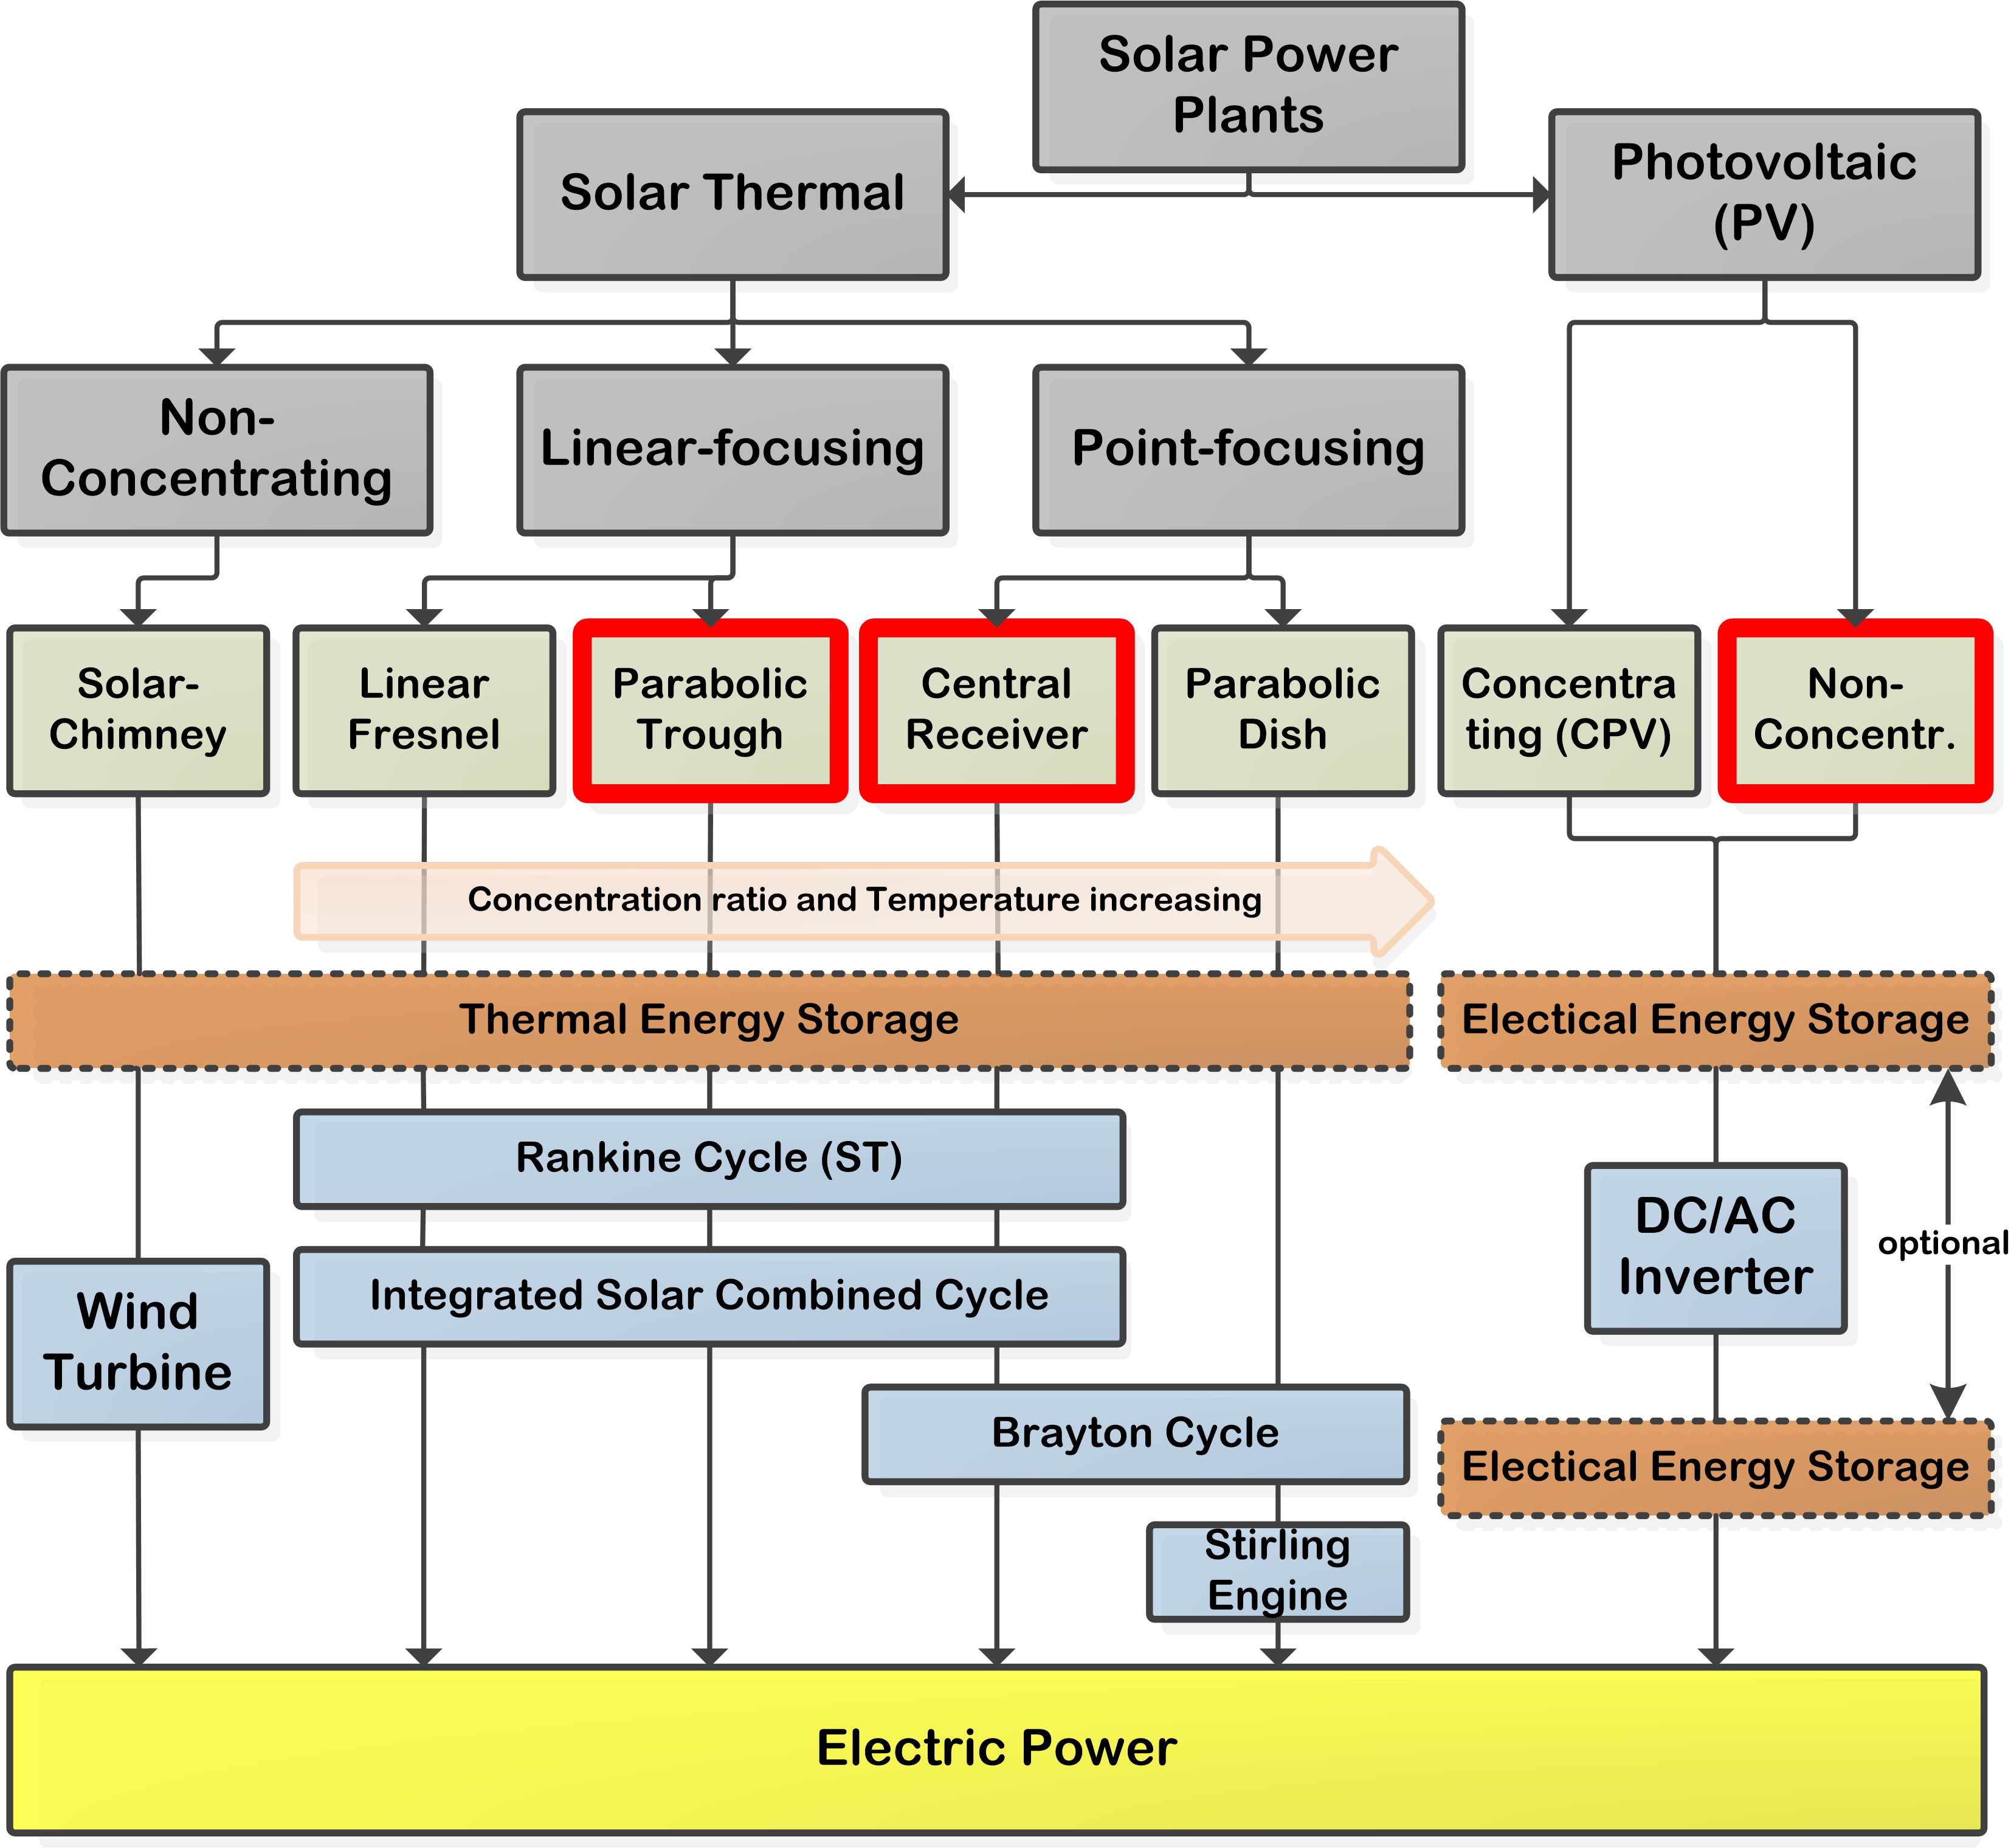
\includegraphics[width=0.8\linewidth]{FIG/OverviewSTP}
\caption[Overview of Solar Power Technologies.]{Overview of Solar Power Technologies.}\label{OverviewSTP}
\end{figure}



%Therefore it is split in the technology fields of large scale concentrated solar power plants (\ref{Large scale concentrated solar power (CSP) plants}) and large scale photo voltaic power plants (\ref{Large scale photo voltaic (PV) power plants}).
%In detail the technologies with a large-scale power plant potential -- parabolic trough, central receiver and non-concentrating photovoltaic -- are described. Also the storage systems for both systems. 
%Therefore it is split in the technology fields of large scale concentrated solar power plants (\ref{Large scale concentrated solar power (CSP) plants}) and large scale photo voltaic power plants (\ref{Large scale photo voltaic (PV) power plants}).
%In detail the technologies with a large-scale power plant potential -- parabolic trough, central receiver and non-concentrating photovoltaic -- are described. Also the storage systems for both systems. 

\section{Large-scale CSP plants}\label{Large scale concentrated solar power (CSP) plants}
%Concentrating solar power (CSP) systems use combinations of mirrors or lenses to concentrate direct beam solar radiation to produce forms of useful energy such as heat, electricity and others. This happens by use of various downstream technologies. Generally the CSP technology includes not only the concentrating solar thermal (CST) technology, but also concentrating photovoltaic (CPV) energy conversion. However, there is no focus on CPV in this thesis. That is why the term CST is put on a level with CSP.
Concentrating solar power (CSP) systems use combinations of mirrors or lenses to concentrate direct beam solar radiation to produce forms of useful energy such as heat and electricity. This happens by use of various downstream technologies. Generally, CSP technology includes not only concentrating solar thermal (CST) technology, but also concentrating photovoltaic (CPV) energy conversion. However, CPV will not be treated in this thesis.
%A CSP plant comprises four main sub-systems: concentrating system, solar receiver, storage and power block. Also supplementary firing is used in some cases, but is basically not necessary nowadays. A graphic scheme of such a sub-system is shown in Figure~\ref{MainComp}. The separate components are linked together by energy flow in mostly radiation transfer or fluid transport. This chapter describes the function and gives an application overview of the individually components. 
A CSP plant comprises four main sub-systems: concentrating system, solar receiver, storage and power block (Figure~\ref{MainComp}). (Supplementary firing was used in the past, but is not necessary nowadays.) The separate components are energetically linked via radiation or fluid transport.
\begin{figure}[!h] 
\centering
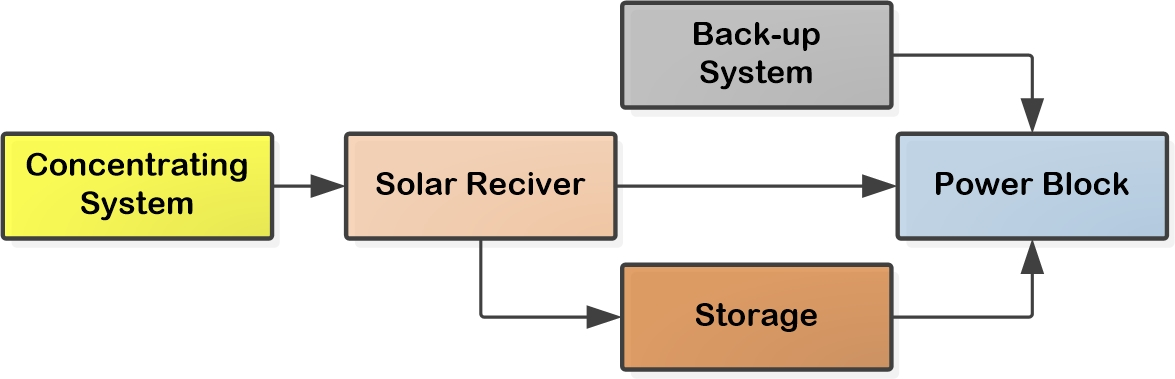
\includegraphics[width=0.85\linewidth]{FIG/MainComp}
\caption[Main components of a CSP plant.]{Main components of a CSP plant.}\label{MainComp}
\end{figure}

%The main advantage of CSP in opposite to other renewable energy producers is the thermal storage to provide power for cloudy days or during night time. Therefore the concentrating system and solar receiver have to produce more thermal energy then the power block can use directly. The ratio of the power capacity of the collector field to the capacity of the power block is defined as Solar multiple (SM). For CSP systems with storage, the number of hours of storage is based on the capacity of the power block. Chapter \ref{Subsection_storage_system} describes technical possibilities and application of thermal storage system for CSP.
The main advantage of CSP when compared to other renewable energy producers is its thermal storage, which continues to provide power on cloudy days or at night. This means that the concentrating system and solar receiver must produce more thermal energy then the power block can use directly. The ratio of the output of the collector field to the gross output of the power block is defined as \emph{solar multiple} (SM). For CSP systems with storage, the number of hours of storage is based on the capacity of the power block.

%The solar receiver or concentrating system is eponymously for the main CST technologies. The two most common CSP plant technologies are parabolic trough collector (PTC) and central receiver (CR) systems (also known as solar power towers). Further types of CSP plant are linear Fresnel reflectors (LFR) and parabolic dish. The main difference of the technologies is the concentrating system. Thereof results the differences in optical design, shape of receiver, nature of the transfer fluid and capability to store heat before it is turned into electricity. In systems with a line focus (PTC trough and LFR) the mirrors track the sun along one axis. In those with a point focus (CR and parabolic dish), the mirrors track the sun along two axes. The receiver may be fixed, as in LFR and CR, or mobile as in PTC and parabolic dish systems. An overview of the technologies and there differences in relation to the focus and the receiver  is shown in Table \ref{tbl: CSPtech}.
The two most common CSP plant technologies are parabolic trough collector (PTC) and central receiver (CR) systems (also known as solar power towers). Other types include linear Fresnel reflector (LFR) and parabolic dish. The main difference between these technologies is the concentrating system, which lead to differences in optical design, shape of receiver, nature of the transfer fluid and capability to store heat before it is turned into electricity. In systems with a line focus (PTC and LFR) the mirrors track the sun along one axis. In those with a point focus (CR and parabolic dish), the mirrors track the sun along two axes. The receiver may be fixed, as in LFR and CR, or mobile as in PTC and parabolic dish systems (see Table \ref{tbl: CSPtech}).

\begin{table}[h!] % Main technologies 
  \centering
  \begin{tabular}{  m{5cm}  m{5cm}  m{5cm}  }
    \hline
    & \textbf{Line focus} & \textbf{Point focus} \\ 
    & Collectors track the sun along a single axis and focus irradiance on a linear receiver. This makes tracking the sun simpler. & Collectors track the sun along two axes and focus irradiance at a single point receiver. This allows for good receiver efficiency at higher temperatures.\\ \hline \hline
    \textbf{Fixed receiver} & &\\

    Fixed receivers are stationary devices that remain independent of the plant's focusing device. This eases the transport of collected heat to the power block.
    &
    \begin{minipage}[t]{5cm}
      \centering
	 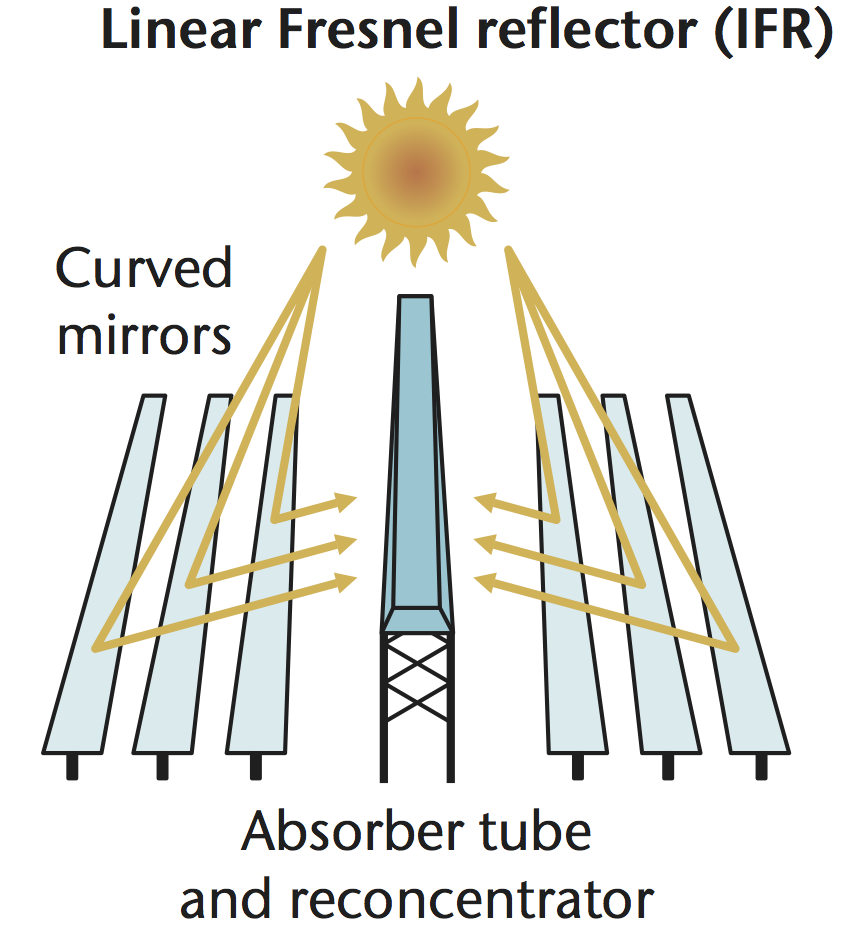
\includegraphics[height=55mm]{FIG/SUM/LF}
    \end{minipage}
    & 
    \begin{minipage}[t]{5cm}
      \centering
	  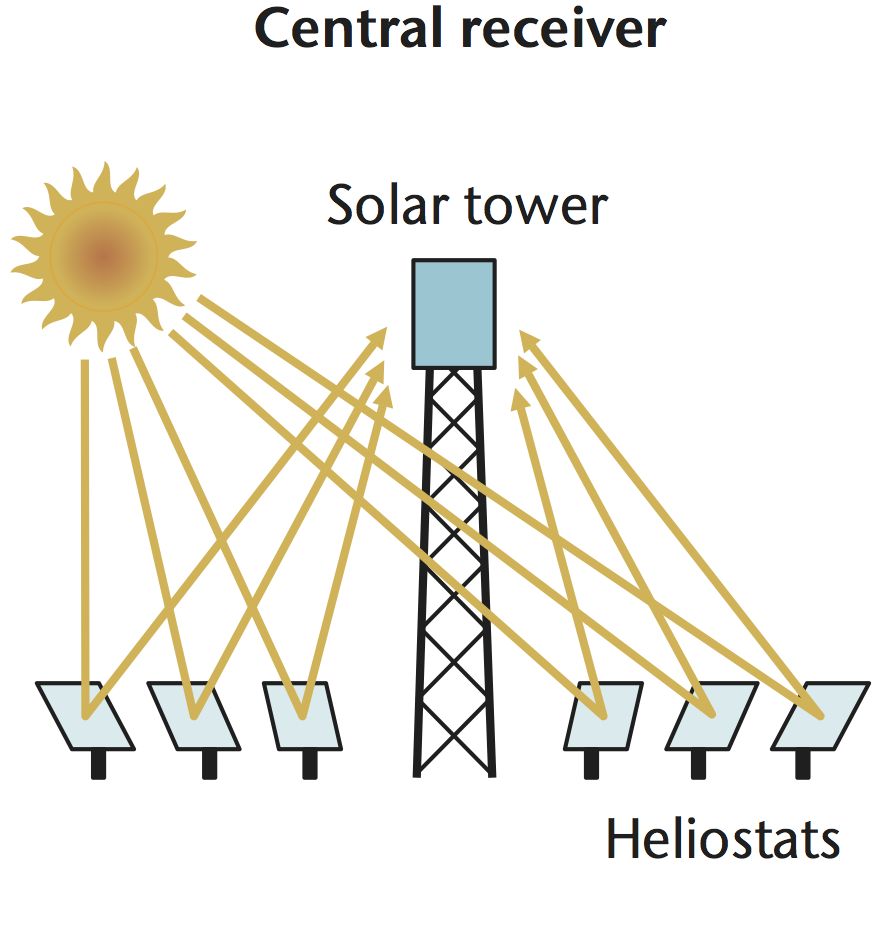
\includegraphics[height=55mm]{FIG/SUM/ST}
    \end{minipage}
    \\ \hline
    \textbf{Mobile receiver} & & \\
    Mobile receivers move together with the focusing device. In both line focus and point focus designs, mobile receivers collect more energy.
    &
    \begin{minipage}{5cm}
      \centering
	  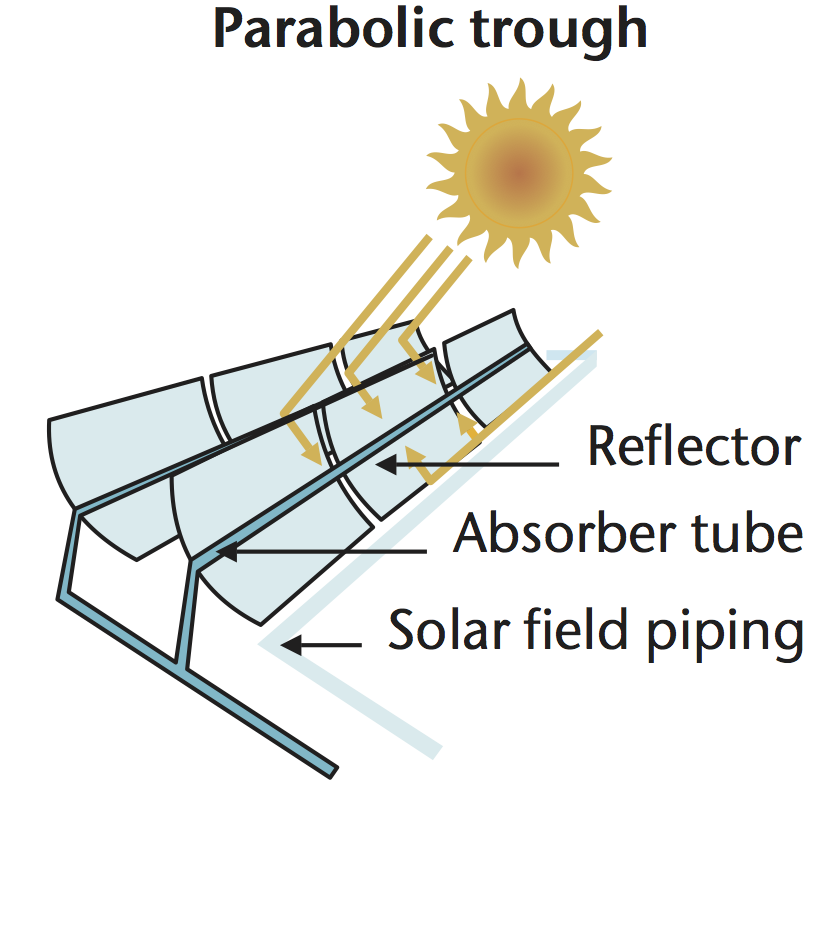
\includegraphics[height=55mm]{FIG/SUM/PT}
    \end{minipage}
    & 
    \begin{minipage}{5cm}
      \centering
	  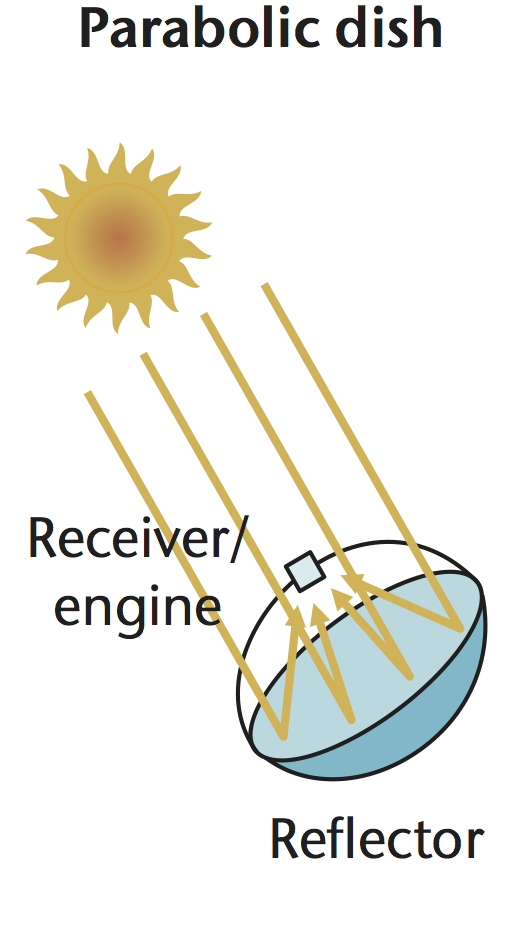
\includegraphics[height=55mm]{FIG/SUM/PD}
    \end{minipage}    
    \\ \hline
  \end{tabular}
  \caption[CSP technology families.]{CSP technology families \cite{IEA2014c}.}\label{tbl: CSPtech}
\end{table}


%As mentioned above is main difference between the CSP technology families how they concentrate the solar radiation. This strongly affects their overall efficiency. The parabolic dish has the best annual optical efficiency (about 90\%) because the concentrator axis is always parallel to the sun rays. The worst (about 50\%) is observed for linear Fresnel systems because of poor performance in the morning and in the evening. Intermediate values (65-75\%) are obtained for parabolic trough and tower systems. For each family the actual efficiency varies with the location, the time of day and the season of the year. \cite{EASAC2011} 
The main difference between the CSP technology families is in how they concentrate the solar radiation, which affects their overall efficiency. The parabolic dish has the best annual optical efficiency (\sim\SI{90}{\percent}) because the concentrator axis is always parallel to the sun's rays. The worst (\sim\SI{50}{\percent}) is observed for linear Fresnel systems because of poor performance at low solar irradiation angles. Intermediate efficiencies (\SIrange{65}{75}{\percent}) are obtained for parabolic trough and central receiver systems. For each family, actual efficiency varies with location, time of day and season \cite{EASAC2011}.

%The capacity range of an CSP-plant is also strongly affected by the concentration ratio. The most common definition of concentration ratio is the ratio of the area of reflector aperture ($A_a$) to the area of receiver ($A_r$). The area concentration is:
The capacity range of a CSP plant is also strongly affected by the concentration ratio, which is defined as the ratio of the area of reflector aperture ($A_a$) to the area of receiver ($A_r$):

\begin{align}
C=\frac{A_{a}}{A_{r}} \label{GL_concentration}
\end{align}
%The concentration ratio from Equation \ref{GL_concentration} has an upper limit that depends on whether the concentration is a three dimensional (point focus) concentrator such as a parabolic dish and central receiver solar tower or a two-dimensional (linear focus) concentrator such as parabolic trough and linear Fresnel reflector. The maximum concentration ratio is based on the second law of thermodynamics applied to radiative heat exchange between the sun and the receiver. The maximum possible concentration ratio for circular concentrators is 45~000, and for linear concentrators is the maximum 212. \cite{Duffie2013}
The concentration ratio from Equation \ref{GL_concentration} has an upper limit that depends on whether the concentration is a three-dimensional (point focus) concentrator such as a parabolic dish or central receiver, or a two-dimensional (linear focus) concentrator such as a parabolic trough or linear Fresnel reflector. The maximum concentration ratio is based on the second law of thermodynamics applied to radiative heat exchange between the sun and the receiver. The maximum possible concentration ratio for circular concentrators is \num{45000}, for linear concentrators it is \num{212} \cite{Duffie2013}.

\begin{table}[h!]  
  \centering
	\begin{tabular}{  p{3.0cm}  C{2.0cm}  C{2.2cm}  C{2.0cm}  C{2.0cm}  C{2.0cm}} 
\hline
\textbf{Technology} & \textbf{Capacity range} (\si{\mega\watt}) & \textbf{Concent- ration} & \textbf{Peak system efficiency} (\si{\percent}) & \textbf{Annual system efficiency} (\si{\percent}) & \textbf{Thermal cycle efficiency} (\si{\percent}) \\ \hline \hline
Parabolic trough & 10-280$^1$ & 70-100 & 21 & 10-16 & 35-42 ST  \\ \hline
Fresnel reflector & 10-200 & 25-100 & 20 & 9-13 & 30-42 ST  \\ \hline
Solar tower & 10-200 &  300-1~000 & 23 & 8-23 & 0-45 ST  \\ \hline
Dish-Stirling & 0.01-0.4 & 1~000-3~000 & 29 & 16-28 & 30-40  \\ \hline
\multicolumn{2}{l}{ST = Steam Turbine}
\end{tabular}
\caption[Performance characteristics of CSP technology families.]{Performance characteristics of CSP technology families \cite{Pitz-Paal.2013} \cite{AbengoaSolar2013a}$^1$.}\label{tbl: CSPCharacteristics}
\end{table}

%But actually the technical implementation of concentration ratio is the main parameter for the capacity range of a CSP plant. Table~\ref{tbl: CSPCharacteristics} gives an overview of some of the performance characteristics of the concentrating solar power concepts. More details are listed in Annexure I, Part A, Figure~\ref{CSPOverview1} on Page~\pageref{CSPOverview1} and Figure~\ref{CSPOverview2} on Page~\pageref{CSPOverview2}. PTC, LFR, and CR can be coupled to steam cycles of 10-280~MW electric capacity (and more), with thermal cycle efficiencies of 30-45~\%. Also the applies for stirling engines which are coupled to dish systems have similar efficiency ranges. The conversion efficiency of the power block remains essentially the same as in conventional-fired power plants. The annual system efficiency are the net power generation over incident beam radiation. They are lower than the conversion efficiencies of conventional steam or combined cycles, because they include the conversion of solar radiative energy to heat within the collector and the conversion of the heat to electricity in the power block. \cite{Pitz-Paal.2013}
% I do not understand the intended meaning of this sentence:
%But actually the technical implementation of concentration ratio is the main parameter for the capacity range of a CSP plant.

Table~\ref{tbl: CSPCharacteristics} gives an overview of performance characteristics. PTC, LFR, and CR systems can be coupled to steam cycles of \SIrange{10}{280}{\mega\watt} electric capacity (and more), with thermal cycle efficiencies of \SIrange{30}{45}{\percent}. Stirling engines that are coupled to dish systems have similar efficiency ranges. The conversion efficiency of the power block is consistent with conventional power plants. The annual system efficiency is the net power generation over incident beam radiation. This is lower than the conversion efficiencies of conventional steam or combined cycles because it includes include the conversion of solar radiative energy to heat within the collector and the conversion of the heat to electricity in the power block \cite{Pitz-Paal.2013}.

\begin{figure}[!h] 
\centering
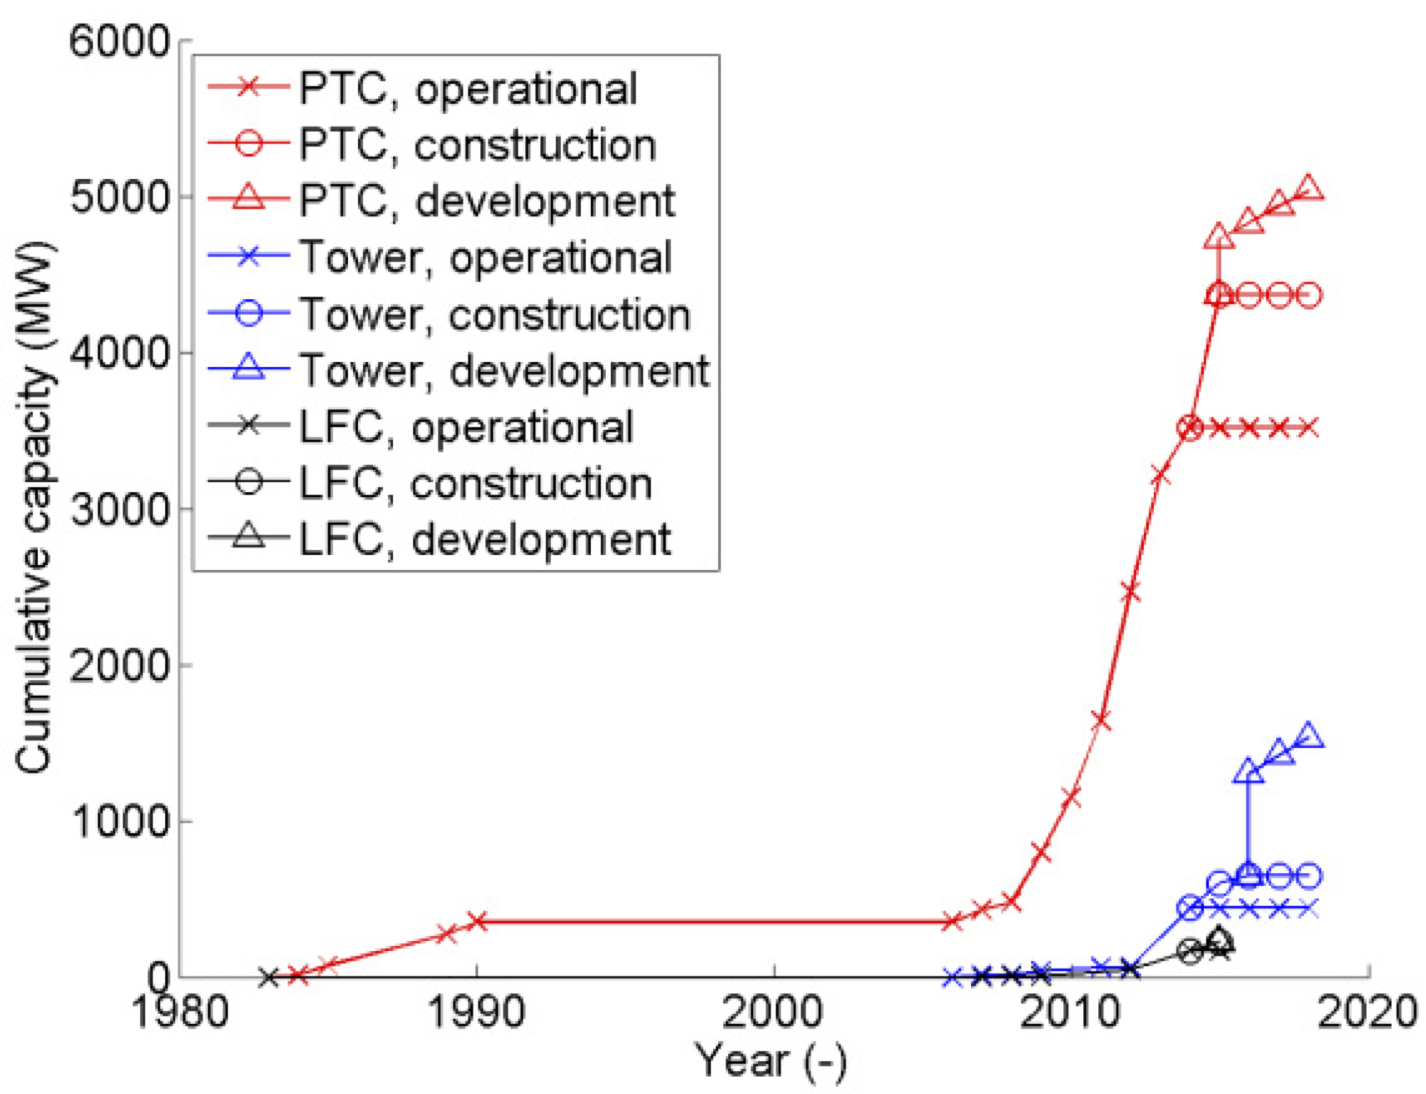
\includegraphics[width=0.65\linewidth]{FIG/CSP_technology_development}
\caption[Historical development of CSP technologies.]{Historical development of CSP technologies \cite{Abbas2015}.}\label{CSP_technology_development}
\end{figure}

%The development of the actual CSP plant technology goes back in the 1970's and 1980's, which is a consequent from the first two Oil crises. Figure~\ref{CSP_technology_development} shows the historical development of PTC, LFR in the Figure called linear Fresnel collector (LFC) and the CR (tower). The parabolic dishes have not succeeded at all and aren't shown here. The reason for that is mainly due to the high structural costs of moving an large diameter dish with two-axes tracking. One might observe that the predominant technology is the PTC, with an installed capacity well above 3~GW. CR have started the exponential development some years later compared to PTC, which explains why the operational installed capacity is much lower. Similarly the development for LFR have started even later, which drives to the lowest installed capacity of the three technologies. The difference in the timing of the three successful technologies is very influenced by the CSP development in its first golden period, the 1980's. In such period important central tower prototypes were built in USA (Solar One, Solar Two, CESA-1) and a 365~MW PTC solar plant was installed in the Mojave Desert. When the oil prices dropped at the end of the second oil crises interest on renewable energies was lost until the last decade. 
The development of the CSP technology began in earnest in the 1970s, a consequence of the first two oil price shocks. Figure~\ref{CSP_technology_development} shows the historical development of PTC and LFR (called linear Fresnel collector (LFC) here) technologies and the CR (tower). Parabolic dish systems have not been widely adopted and are not shown here; this is mainly due to the high costs associated with moving a large diameter dish with two-axis tracking. The predominant technology remains PTC, with an installed capacity well above \SI{3}{GW}. The first commercial-scale CR systems were built decades later, and that of linear Fresnel reflector systems later still; the operational installed capacity is proportional to the number of years the technology has been available. In the 1980s, important central tower prototypes were built in the USA (\emph{Solar One}, \emph{Solar Two}, \emph{CESA-1}) and the \SI{365}{\mega\watt} PTC solar plant was built at Kramer Junction in the Mojave Desert. When oil prices dropped after the second oil crisis, interest in renewable energies waned and did not return until the beginning of the new millenium. 

%With regard to the past development in the different CSP technology deals this theses with the PTC as well as with the CR technology. The most relevant facts to the separate technologies and there technical components are described in the following shortly in order to describe there technical possibilities to cover the prescribed load curve. 

This work treats PTC and CR technology. Relevant features of these technologies and their technical components are described here briefly, as they have implications for a plant's ability to meet the prescribed load curve. 

\subsubsection{Overview of CR system technology}
%As it was mentioned above, a CSP system basically consists of five main part, namely concentration system, solar receiver, storage, power block and heat transfer fluid (HTF) system. Which are in case of a CR power plant a solar field (heliostat field) consisting by several two-axis tracking heliostats, a thermal receiver which is mounted on a tower, a thermal storage usually using molten salt or a steam accumulator (depending on HTF), a power block mostly based on Rankine cycle technology and steam or molten salt as HTF. Figure~\ref{towerdirecttwotank} shows the simplified CR power plant scheme of the demonstration project \emph{Solar Two} (1995-2001). 

A CSP system consists of five main components: the concentration system, solar receiver, storage, power block and heat transfer fluid (HTF) system. In the case of a CR plant, these are, respectively, a solar field (heliostat field) consisting by several two-axis tracking heliostats, a thermal receiver which is mounted on a tower, thermal storage usually using molten salt or a steam accumulator (depending on HTF), a power block based on Rankine cycle technology, and steam or molten salt as HTF (Figure~\ref{towerdirecttwotank}).

%Currently CR systems can be separated by two receiver types, external (tube) receiver and cavity receiver \cite{Hoffschmidt2014}. The \emph{Solar Two} project used a external receiver to heat up molten salt at a top temperature of \SI{565}{\celsius} \cite{Reilly2001}. This project concept was the basic research for the current state of art in CR power plants using molten salt as HTF. Typical solar heat fluxes in this type of receiver are up to \SI{1}{\mega\watt\per\square\metre} \cite{Pitz-Paal.2013}. Cavity receiver are currently mostly used in connection with direct saturated or super heated steam production, which is not easy to store over longer duration and therefore not suitable for the defined load profile in thesis \cite{Hoffschmidt2014,Steinmann2015}.

Central receiver systems can be differentiated by type, external (tube) receiver and cavity receiver \cite{Hoffschmidt2014}. The \emph{Solar Two} project used a external receiver to heat up molten salt to \SI{565}{\celsius} \cite{Reilly2001}. This concept is the state of the art for CR plants using molten salt as HTF. Typical solar heat fluxes in this type of receiver are up to \SI{1}{\mega\watt\per\square\metre} \cite{Pitz-Paal.2013}. Cavity receivers are primarily used in connection with direct saturated or super-heated steam production, which is not easy to store over longer duration and therefore not suitable for the prescribed load profile \cite{Hoffschmidt2014,Steinmann2015}.


\begin{figure}[htbp]  
\centering
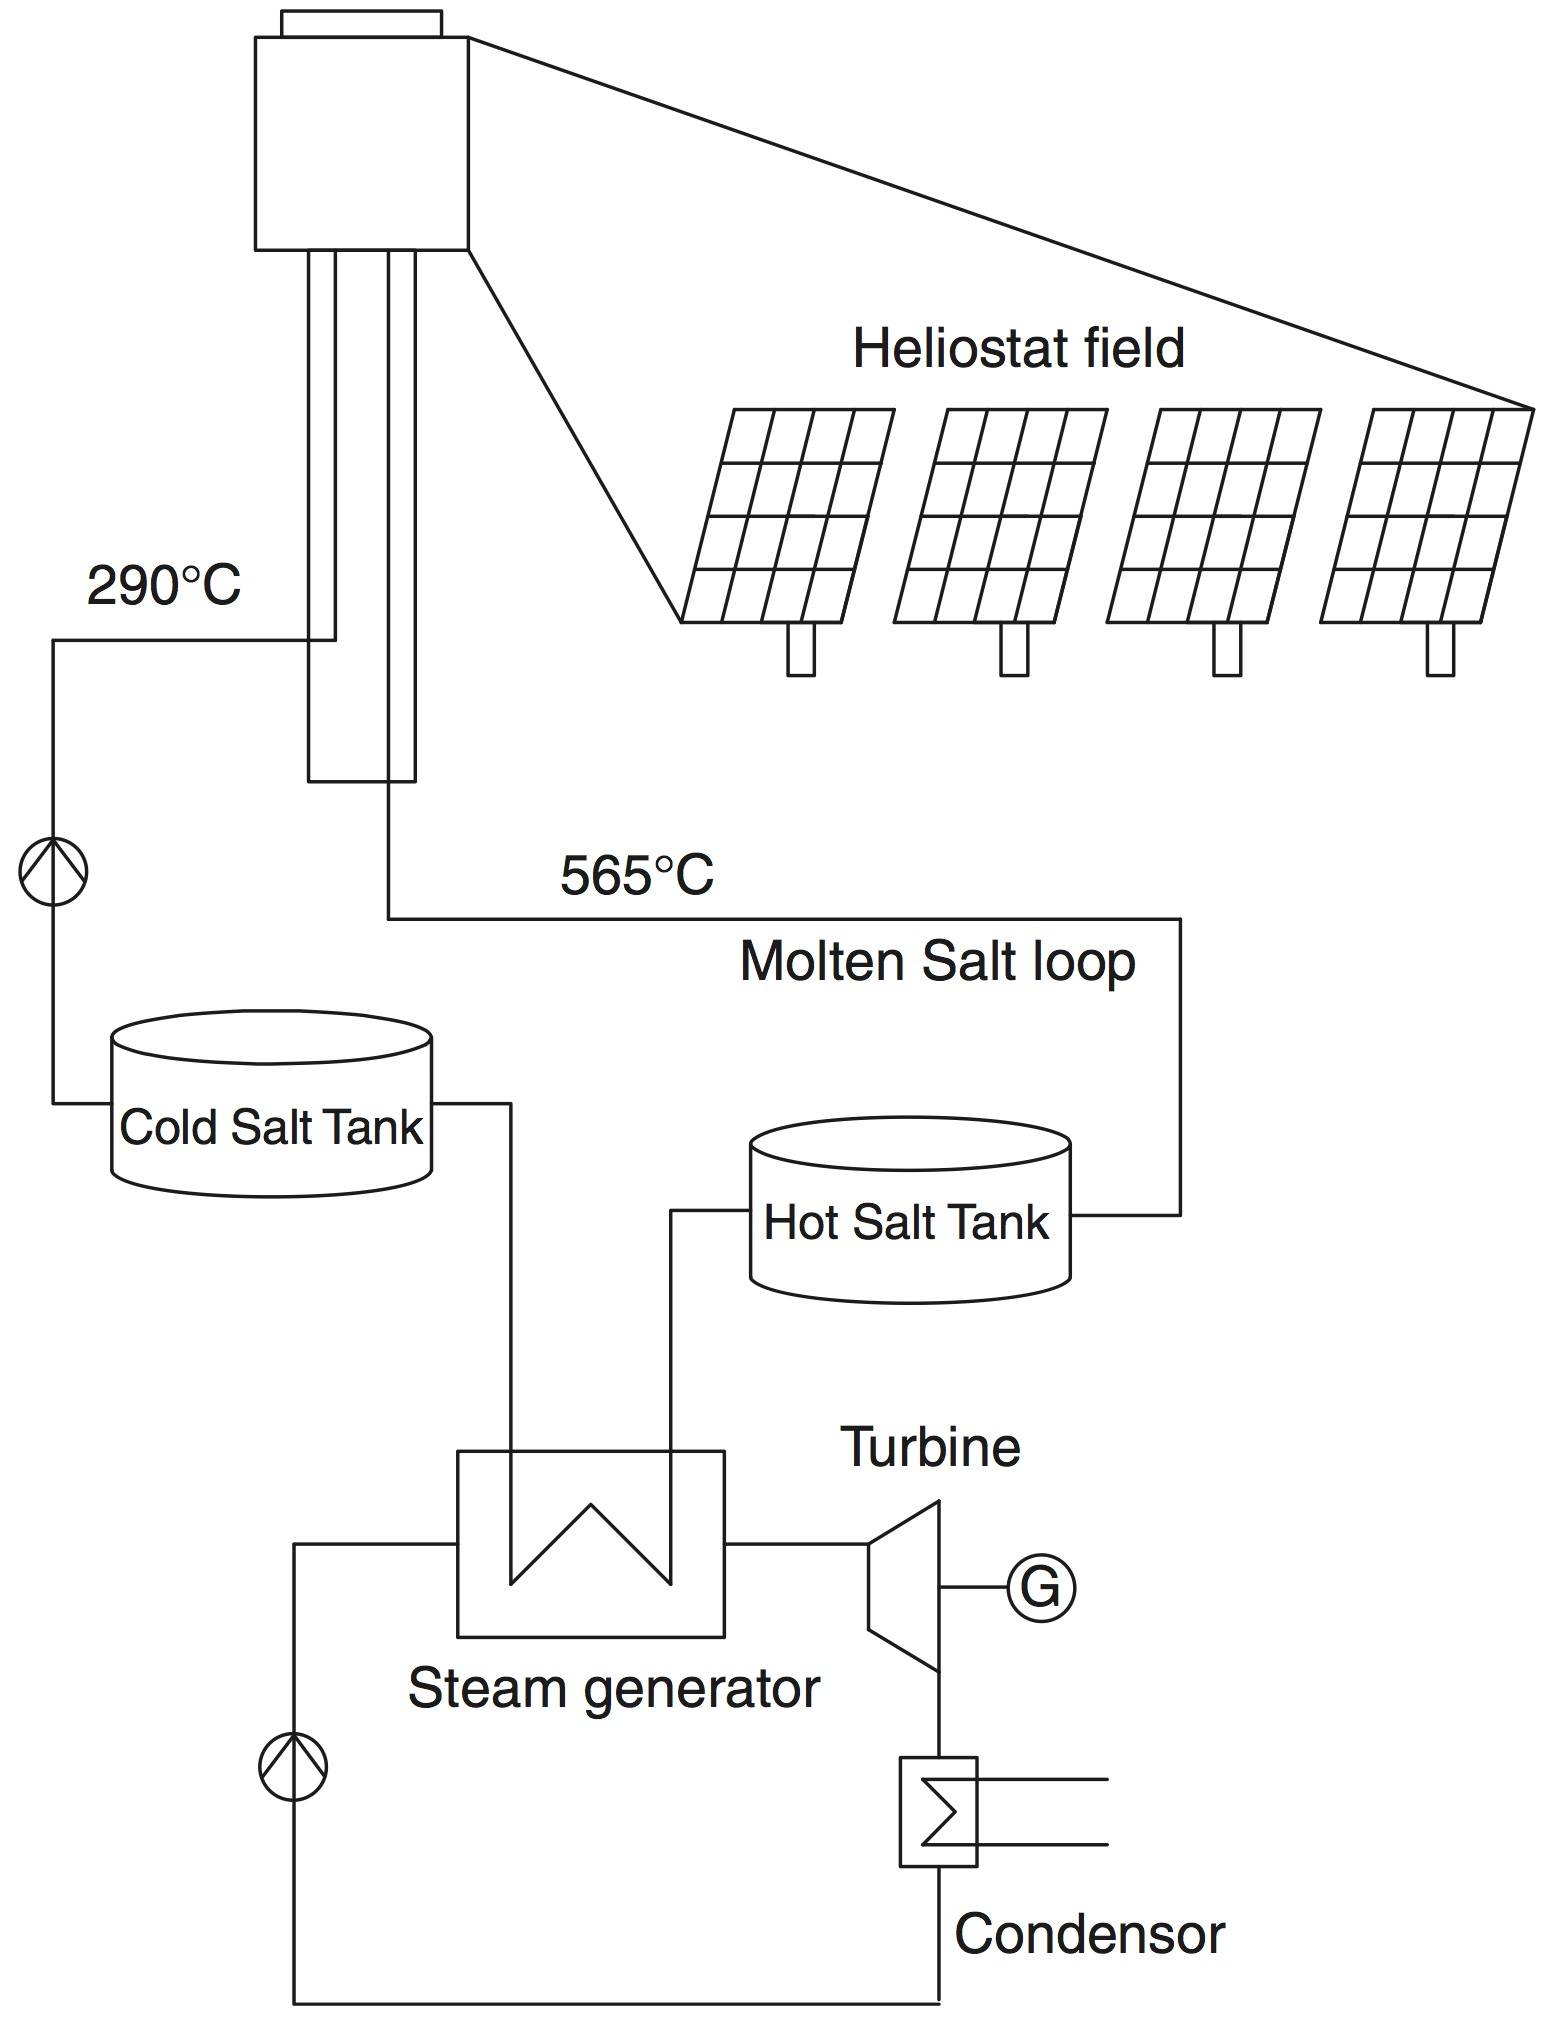
\includegraphics[width=0.45\linewidth]{FIG/towerdirecttwotank}
\caption[Simplified scheme of \emph{Solar Two} CR power plant with direct storage of molten salt used as heat transfer fluid.]{Simplified scheme of \emph{Solar Two} CR power plant with direct storage of molten salt used as heat transfer fluid \cite{Richter2013}.}\label{towerdirecttwotank}
\end{figure}

Classical two-axis tracking heliostats design is dominated by mirrors brought into position by steel structures and drives that guarantee high accuracies underwind loads and thermal stress situations \cite{Alexopoulos2013}. The reflective surface of can therefore reach sizes from \SIrange{1.1}{320}{\square\metre} \cite{Blackmon2012,Tyner2014}. There is not really one specific size pushed through for commercial scale application, but one of the marked leader \emph{Abengoa Solar} currently uses \SI{140}{\square\metre} heliostats for CR projects in SA \cite{Abengoa2014}.

The main advantage for using molten salt as HTF is the comparatively high thermal range and its good manageability storage characteristics. Molten salt in CR systems can be stored directly in two tanks as its shown in the scheme. For the storage capacity, the thermal range of the receiver temperature and the storage volume is decisive. The storage capacity is usually measured in hours of storage capacity at full load turbine output. Commercial direct molten salt thermal energy storages (TES) in CR systems currently reaches storage capacities of \SI{17.5}{\hour} \cite{NREL2015b}.

\subsubsection{Overview of PTC system technology} 
The concentration system of a PTC plant consist out of parabolic shaped mirrors which is focusing the solar beam on to a receiver tube in the focus point of the parabola. Commonly synthetic oil is used as HTF which flows through the receiver tube (also known as heat collecting element (HCE)). From the receiver, the heat up synthetic oil gets either transported to the power block or to a TES. The PTC system technology currently also uses mostly molten salt as storage fluid, but indirect due to the different used fluids of storage and solar field. Figure~\ref{troughtindirecttwotank} shows a simplified scheme of the currently most used PTC system.

\begin{figure}[htbp]  
\centering
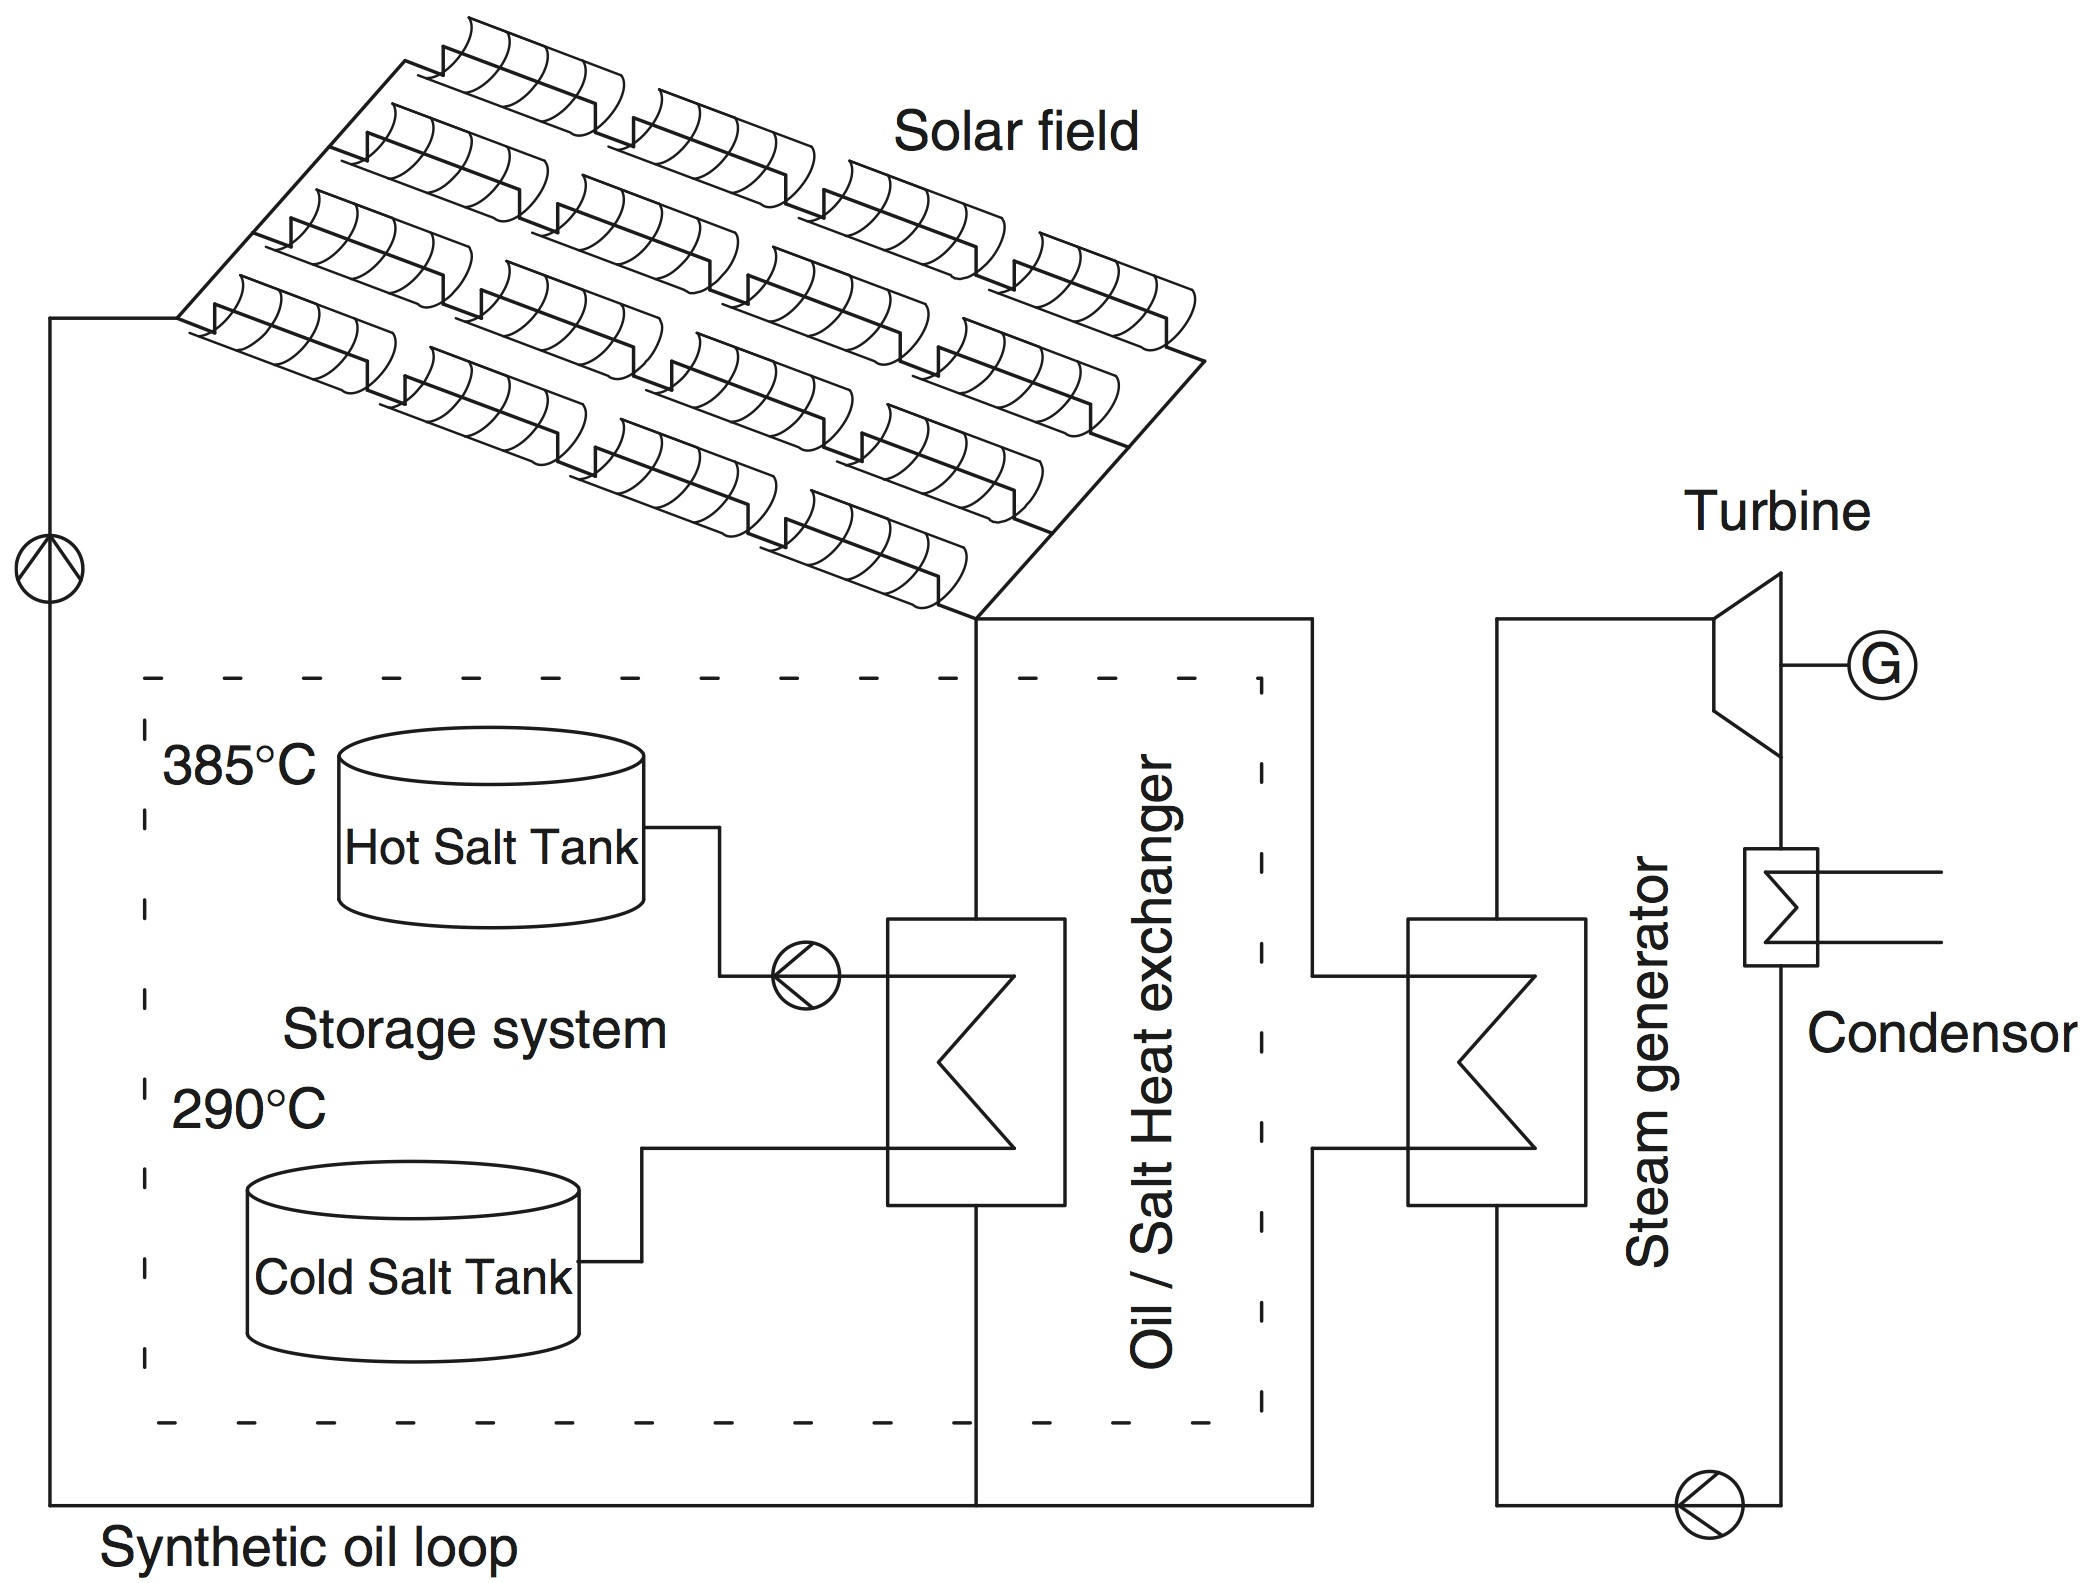
\includegraphics[width=0.65\linewidth]{FIG/troughtindirecttwotank}
\caption[Simplified scheme of PTC power plant with indirect storage system.]{Simplified scheme of PTC power plant with indirect storage system \cite{Steinmann2012}.}\label{troughtindirecttwotank}
\end{figure}
The parabolic shaped mirrors and the HCE are typically assembled on a support structure mounted on a series of aligned pylons. The center pylon is equipped with a hydraulic drive system to allow tracking of the total solar collector assembly (SCA). Figure~\ref{SCA_EuroTrough} shows a SCA exemplary by using the EuroTrough system. The solar field of a PTC system consists of one or more parallel loops of SCAs. A common header pipe provides each loop with an equal flow rate of HTF. A second header collects the hot HTF to return it either directly to the power cycle or to the TES. \cite{Lupfert2013,Maccari2015}

\begin{figure}[htbp] 
\centering
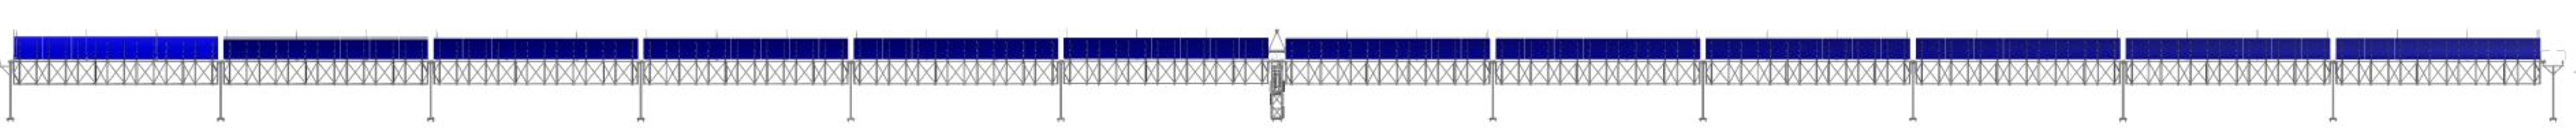
\includegraphics[width=1\linewidth]{FIG/SCA_EuroTrough}
\caption[Typical solar collector assembly composed of 12 EuroTrough collector elements.]{Typical solar collector assembly (SCA) composed of 12 EuroTrough collector elements \cite{VonReeken2014}.}\label{SCA_EuroTrough}
\end{figure}
Current collector sizes varied from \SIrange{2.55}{8}{\metre}, but in order to reduce the total costs of PTC systems the trend for commercial scaled collector sizes is increasing. \cite{AbengoaSolar2013b,Pitz-Paal.2013,VonReeken2014}

All commercial scale PTC systems uses actually oil based HTF. The first commercial used PTC power plant \emph{SEGS-1}, built 1984 in California, uses a mineral oil as HTF in the HCE, which heats up from \SIrange{240}{305}{\celsius}. The upper temperature end for a stable use of mineral oil is around \SI{300}{\celsius}. In order to increase the maximum process temperature actual PTC systems uses synthetic oil with a maximum working temperature of \SI{400}{\celsius}. \cite{Gil2010,Richter2013,Therminol2015}

Synthetic oil is quite expansive therefore it is not used as fluid for TES aplication. Molten salt is more than ten times less expansive, that's the main reason why it is currently used as storage medium in the TES of PTC systems \cite{Gil2010}. 

There is a huge research and development expenses for using molten salt also as HTF in the HCE for PTC systems, but currently there are no commercial scale PTC power plants projects with molten salt applications as HTF known. \cite{Maccari2015}

At this stage it can be noted, that PTC uses a lower thermal process temperature than the CR systems, which effects on the one hand the efficiency of the thermal process (Rankine cycle) and on the other hand the required dimensions of the TES medium. 

Furthermore must be noted that the power output of a PTC plant is more effected by the seaseonal variation of the irradiance angle due to not traking the sun in two axis and a thereby resulting higher cosine efficinetcy loss. \cite{Jorgenson2013}

\pagebreak
\section{Large-scale PV power plants}\label{Large scale photo voltaic (PV) power plants}
PV cells are semiconductor devices that convert solar irradiance due to the photovoltaic effect directly into direct current (DC).
Grid-tied systems require inverters to transform DC power in alternating current (AC). Therefore it is in the nature of PV systems that the generate power just during daytime. To support the South African system load even at the most critical time - the evening hours - the PV system needs a storage opportunity for electrical power. Such an electrical energy storage (EES) could either be DC- or AC-site connected with the PV system depending on the EES technology. Figure~\ref{PVMainComp} shows a with a EES extended feasible PV plant scheme.

\begin{figure}[!h] 
\centering
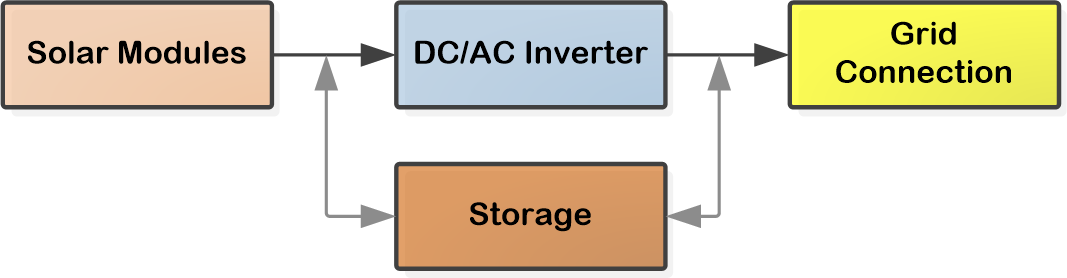
\includegraphics[width=0.75\linewidth]{FIG/PVMainComp}
\caption[Main components of feasible a PV plant.]{Main components of feasible a PV plant.}\label{PVMainComp}
\end{figure}
Such a PV plant scheme is currently not in a commercial use and is therefore more of theoretically nature. Nevertheless with this schema the covering of the prescribed load curve is conceivable.
\subsubsection{Large-scale PV systems}
As it was said above, PC cells generates electricity in form of DC power. The cells are interconnected to form modules, which are then combined to form arrays and systems. PV can be used in various applications with capacities from less then one watt up to hundreds of megawatts. The balance of system (BOS) of grid-tied PV systems includes inverters, transformer, wiring and monitoring equipment, as well as structural components for installing modules.  

Crystalline silicon (c-Si) modules, whether single- (sc-Si also known as mono-Si) or multi-crystalline (mc-Si also known as multi-Si), largely dominate the PV-market. Cells are usually sliced from ingots or castings of highly purified silicon. The manufacturing process creates a potential junction, deposits an anti-reflective costing and adds metal contacts. Cells are then grouped into modules with a transparent glass for the front, a weatherproof material for the back and often a rounded by a frame. Modules are usually guaranteed for a lifetime of 20 years at minimum \SI{80}{\percent} of there rated output, and sometimes at \SI{70}{\percent} for 30 years. In the last 10 years, the efficiency of average commercial silicon modules increased from about \SIrange{12}{16}{\percent}, while the record lavatory cell efficiency is currently \SI{25.6}{\percent} for sc-Si and \SI{20.8}{\percent} for mc-Si wafer-based technology. \cite{FraunhoferISE2015}

Two main alternative solar cell commercial technologies exist: multi-junction cells, used in CPV (will not be dealt with any further) and thin films, based on either amorphous silicon (a-Si), cadmium-telluride (CdTe), copper-indium-(di)selenide (CIS), copper-indium-gallium-(di)selenide (CIGS) or copper-zinc-tin-sulfide \cite{IEA2014c}. The highest lab efficiency in thin film technology is \SI{21.0}{\percent} for CdTe and \SI{20.5}{\percent} for CIGS solar cells. The efficiency of average commercial CdTe module increased from \SIrange{9}{13}{\percent} in the last 10 years \cite{FraunhoferISE2015}.

PV is a fast growing market as it can be seen in Figure~\ref{PV_Prod_by_Tech}. A global installing rate of about \SI{130}{\mega\watt} new PV systems per day should therefore be expected for 2014. The Compound Annual Growth Rate (CAGR) of PV installations was \SI{44}{\percent} between 2000 to 2014 \cite{FraunhoferISE2015}. 

 \begin{figure}[htbp]  
\centering
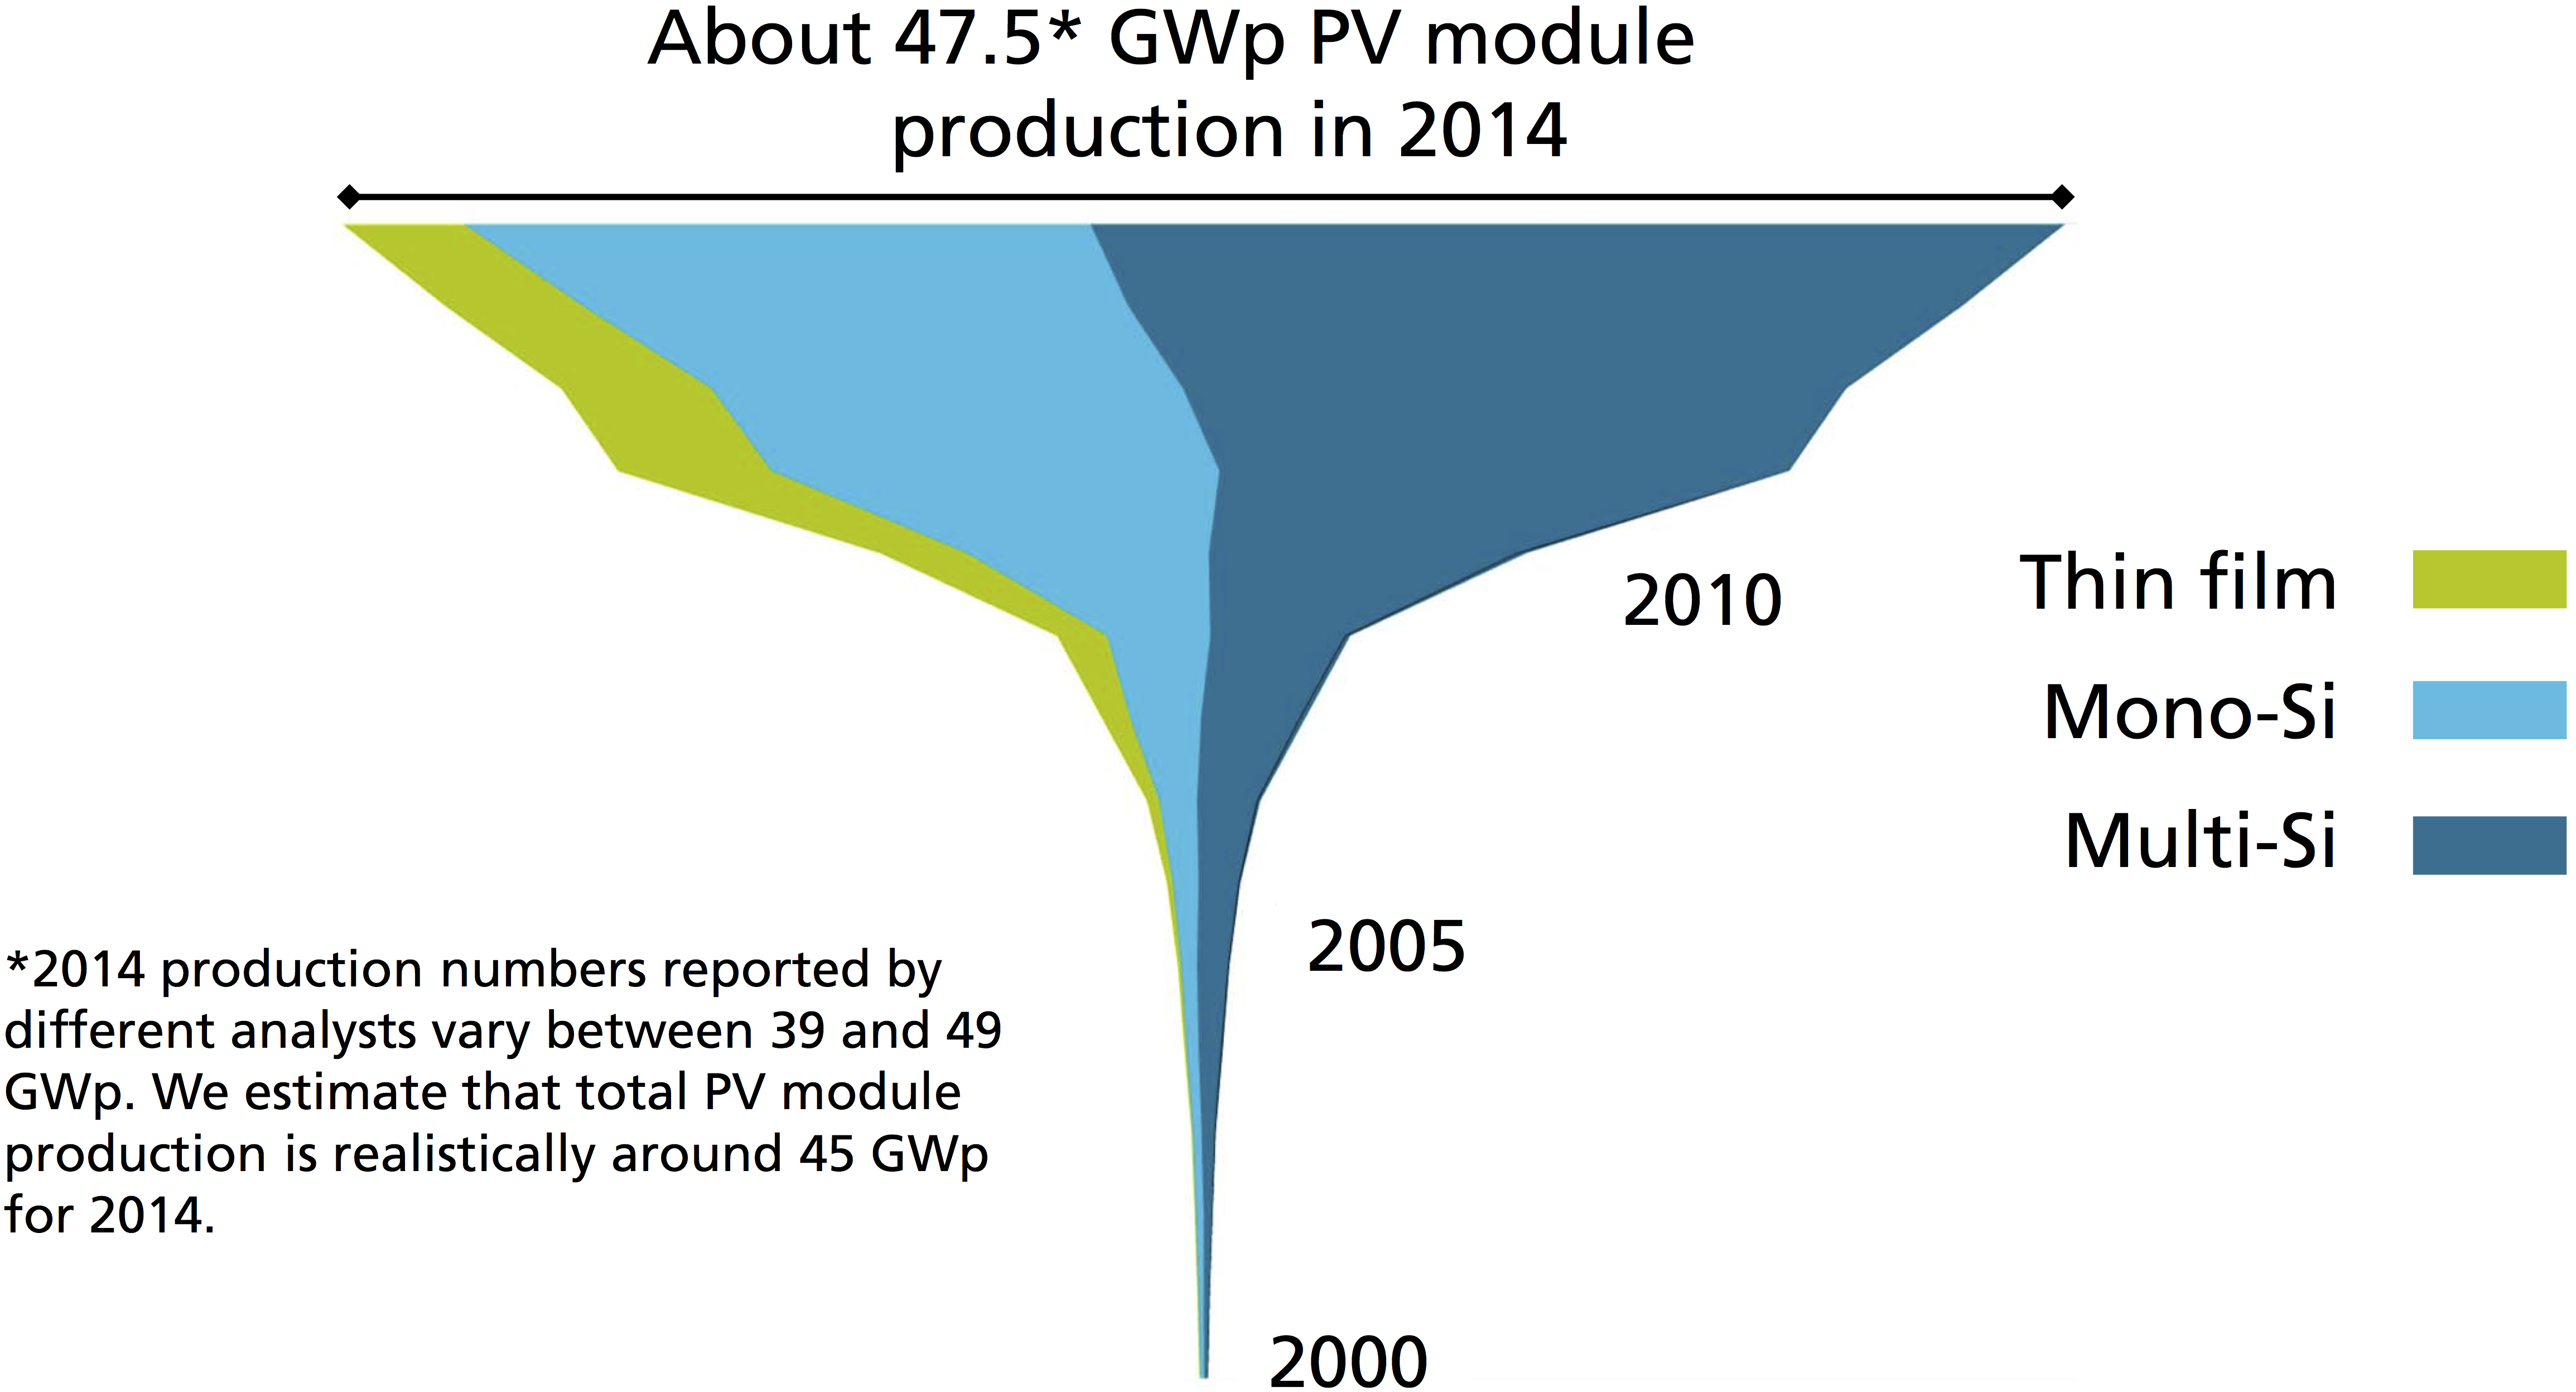
\includegraphics[width=0.7\linewidth]{FIG/PV_Prod_by_Tech}
\caption[Worldwide annual PV production by technology.]{Worldwide annual PV production by technology in \si{\giga\watt}\textsubscript{p} \cite{FraunhoferISE2015}.}\label{PV_Prod_by_Tech}
\end{figure}
Since 2010 the world has added more PV capacity than it had in the previous four decades \cite{IEA2014c}. In 2014 the worldwide installed cumulative PV capacity was about \SI{183}{\giga\watt}\textsubscript{p} whereof \SI{21}{\percent} are allocated Germany. About \SI{80}{\percent} of the actually worldwide cumulative installed PV capacity is assigned to Europe and Asia. Figure~\ref{PV_Install_global} shows the development of the worldwide cumulative installed PV capacity from 2008 to 2014. \cite{FraunhoferISE2015}

\begin{figure}[htbp]  
\centering
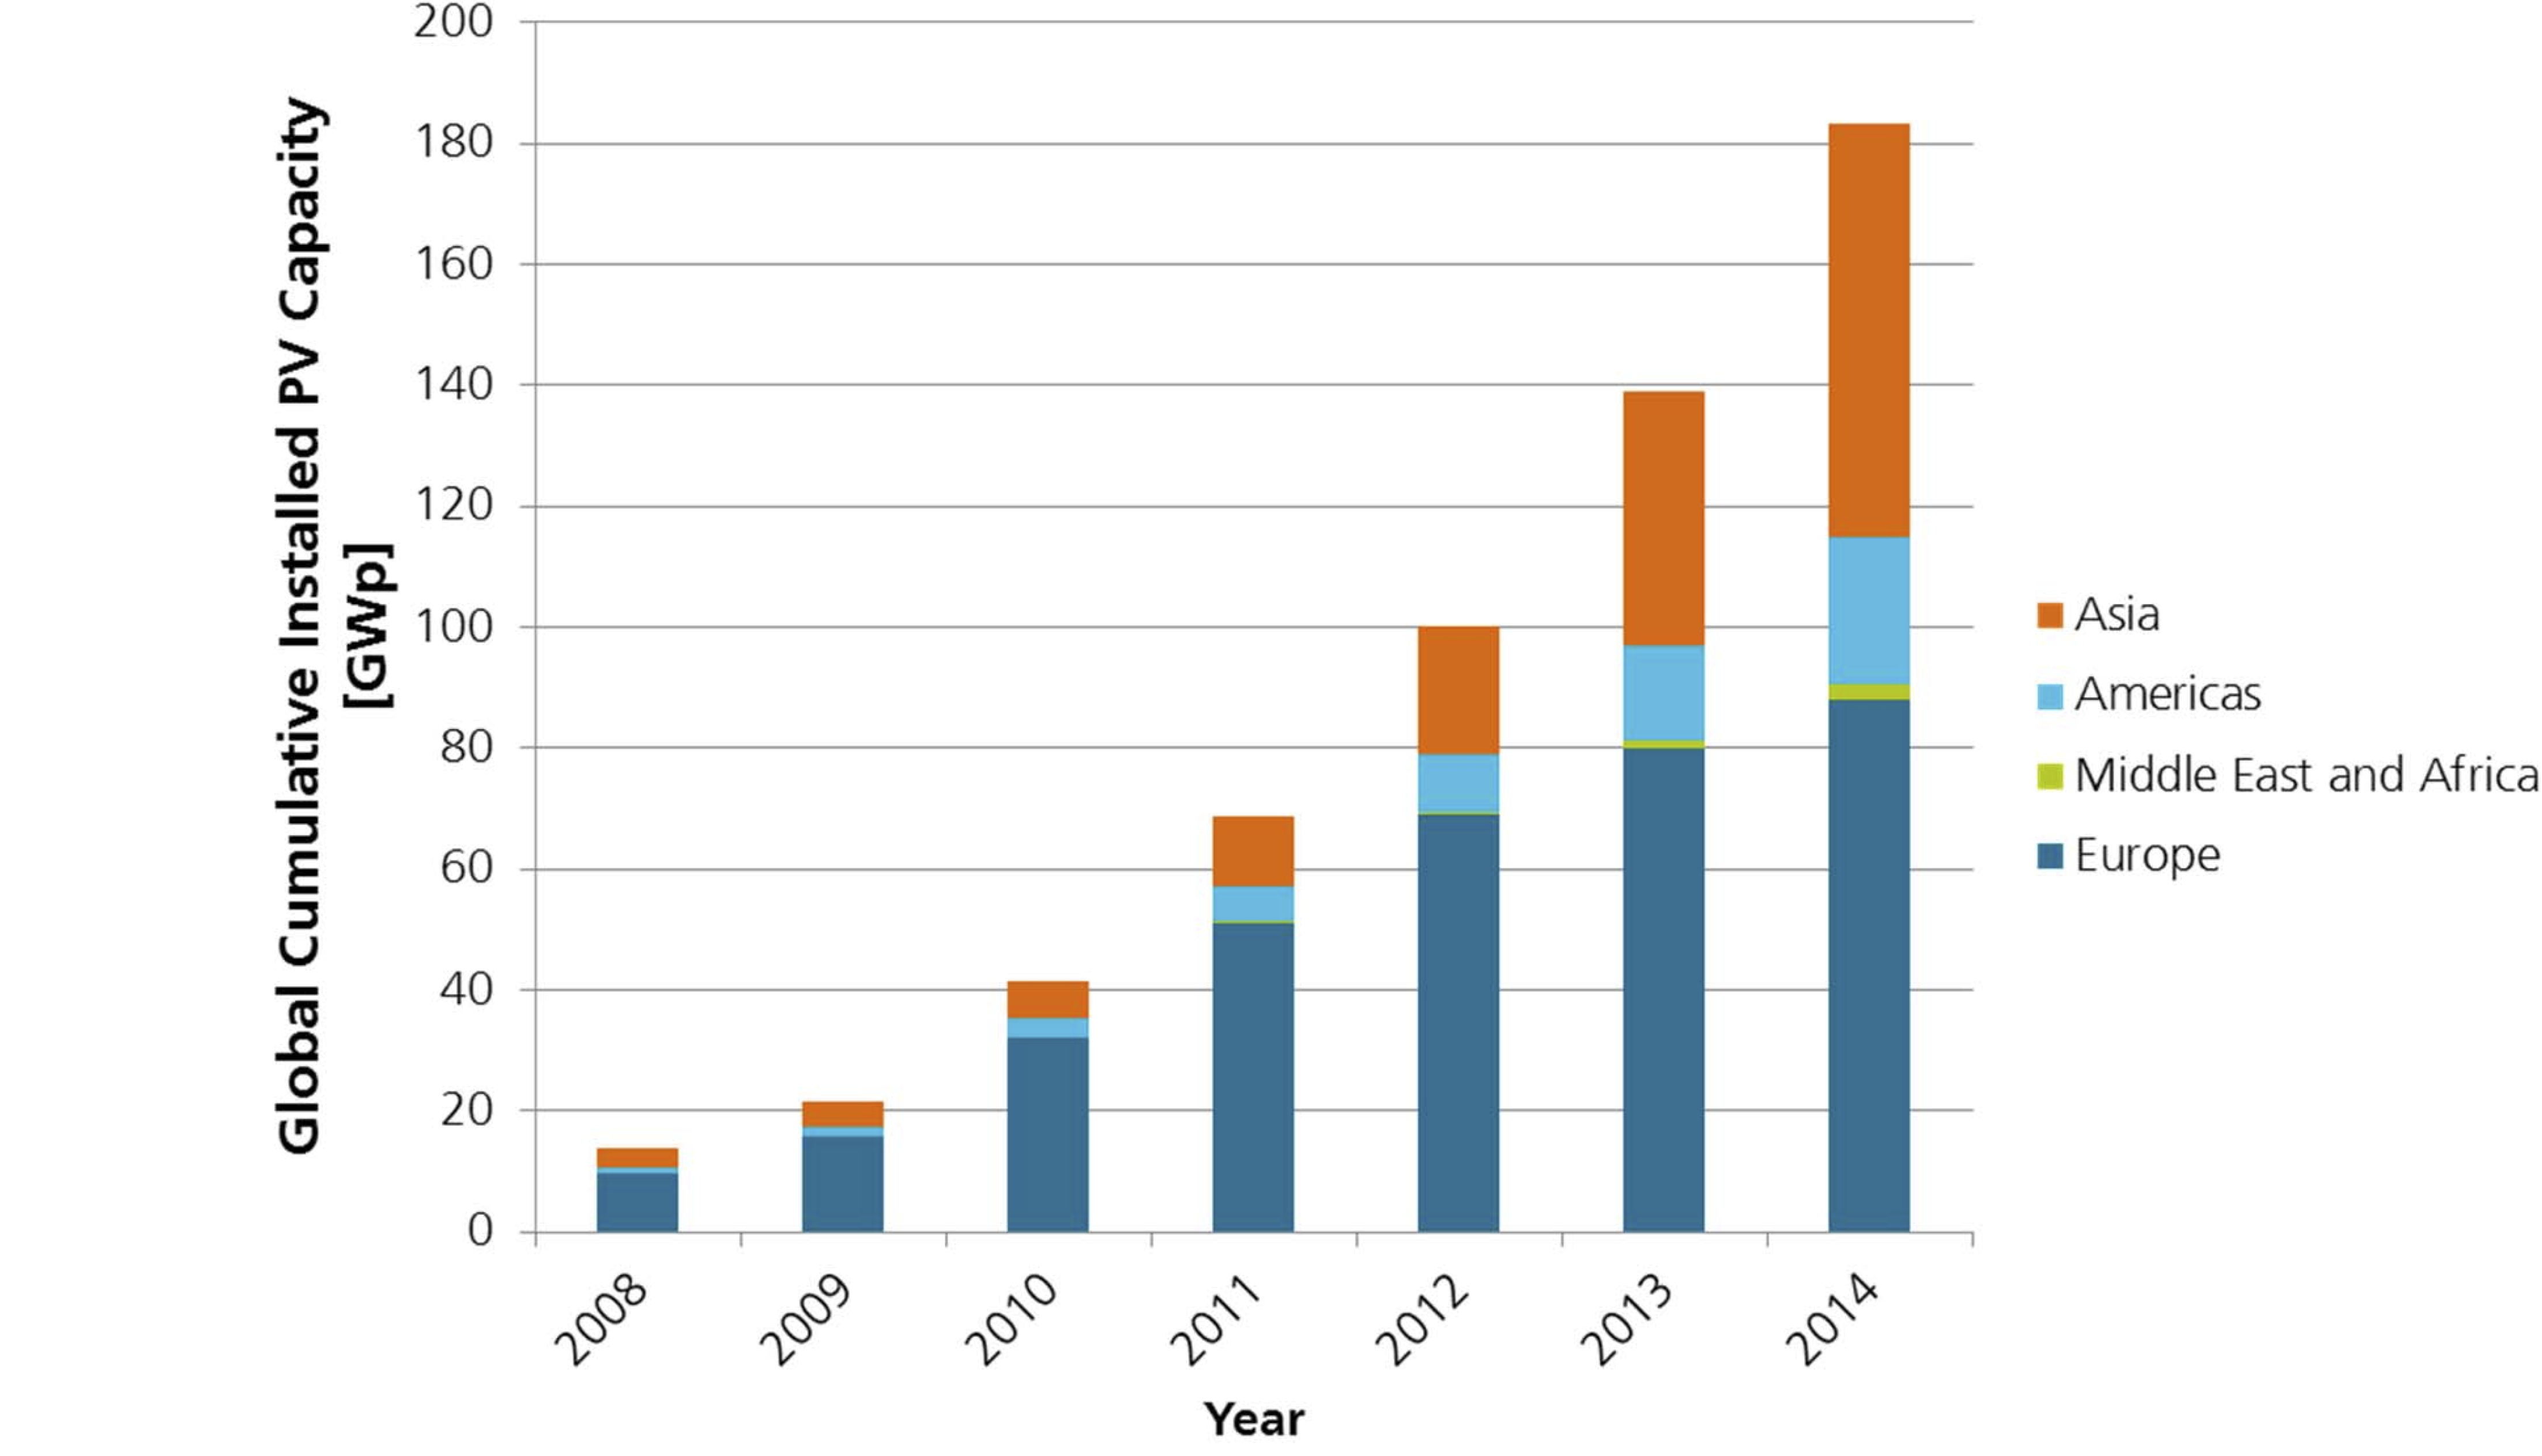
\includegraphics[width=0.7\linewidth]{FIG/PV_Install_global}
\caption[Worldwide cumulative PV installation until 2014.]{Worldwide cumulative PV installation until 2014 \cite{FraunhoferISE2015}.}\label{PV_Install_global}
\end{figure}
The emergence of the global PV market has stimulated rapid cost reductions of modules and systems. In the last few years, intense competition and global over capacities led many PV cell and module manufacturer to price their products too low for investment cost recovery, and thereby several companies failed. 

In 2013 PV systems cost about \SIrange{30}{44}{\percent} what they cost in 2008 (see Figure~\ref{PVsystemCosts}). Prices for PV systems are more diversified than for cells and modules, which tend to be global commodities. Small systems, such as rooftop, are more expansive than larger ones, especially ground-based, unity-scale systems. The prices for the different system types varies significantly among countries. Most of the gap comes from differences in "soft costs", which includes permitting, inspection, interconnection and labour costs \cite{IEA2014c}. Therefore it is important to use country-specific prices for calculating costs.

\begin{figure}[htbp]  
\centering
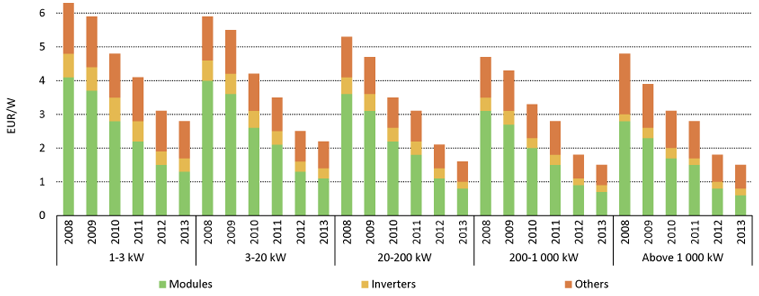
\includegraphics[width=1\linewidth]{FIG/PVsystemCosts}
\caption[PV system cost development by size.]{PV system cost development in Italy by size \cite{IEA2014c}.}\label{PVsystemCosts}
\end{figure}
Installations for unity-scale PV systems in SA currently has a similar cost distribiution then it is shown actually in Itally. Modules makes in SA a share of \SI{37}{\percent} of the total investment cost, while it is \SI{40}{\percent} in Italy. The share of Inverter costs makes \SI{10}{\percent} in SA and \SI{13}{\percent} in Itally. Therefore it can be noteced that the share of further soft costs is higher for unity-scale PV systems in SA then in Italy and makes more than the half of installation costs. \cite{IEA2014c,Terblanche2015}
\pagebreak
\subsubsection{Large-scale electrical energy storage systems}
For supplying the in Section~\ref{SystemloadinSA} prescribed load curve even due to night time the PV system needs assistance by a EES. In generally can be said that a EES consists by two main sections, namely the power conversion system (PCS) and the energy storage unit. A PCS is used to adjust the voltage, current, and other power characteristics of the storage based on the load requirements. PCS may consist of two separated units for charging and discharging with different characteristics. Energy storage section is the other part of EES that is designated to contain the storage medium, e.g. water reservoirs in pumped hydroelectric storage (PHS). Because PCS and energy storage units have inherent inefficiencies and losses, overall efficiency of EES technologies is defined by Equation~\ref{Overall storage efficiency}, in which $E_{out}$ and $E_{in}$ are output and input electric energy, respectively \cite{Kaldellis2009}.
\begin{equation}
\textrm{Overall storage efficiency}=\frac{E_{out}}{E_{in}} \label{Overall storage efficiency}
\end{equation}
Figure~\ref{TCC_EES} illustrates the main sections of a typical EES system and the associated losses.

\begin{figure}[htbp]  
\centering
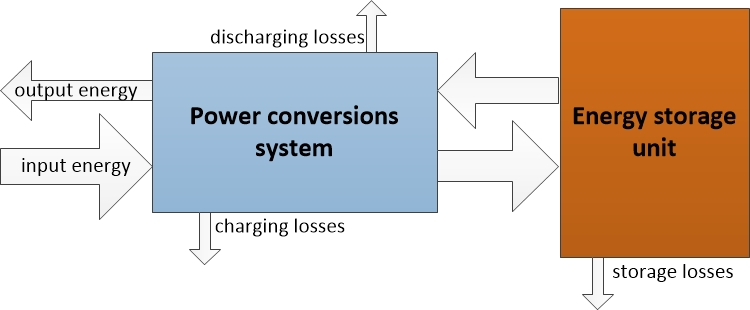
\includegraphics[width=0.65\linewidth]{FIG/EESSchema}
\caption[Main sections of electrical energy storage system and there energy losses.]{Main sections of electrical energy storage (EES) system and there energy losses.}\label{TCC_EES}
\end{figure}
In 2014 the global large-scale energy storage capacity was more than \SI{140}{\giga\watt} of which about \SI{97}{\percent} was allocated by PHS. Rapid deployment of wind and solar PV energy has led to integrate challenges and the need for more flexible storage opportunities. Thereby also alternative grid connected energy storage concepts are growing. Between 2005 and 2014 there was a sharp increase in global capacity of large-scale battery storages from \SIrange{120}{690}{\mega\watt}. Figure~\ref{EESgridCapacity} describes the global capacity development for grid connected storage. It must be noted, that the thermal storage share in this chart also includes decentralized hot water boilers, which is not to be confused with TES of CSP applications.

\begin{figure}[htbp]  
\centering
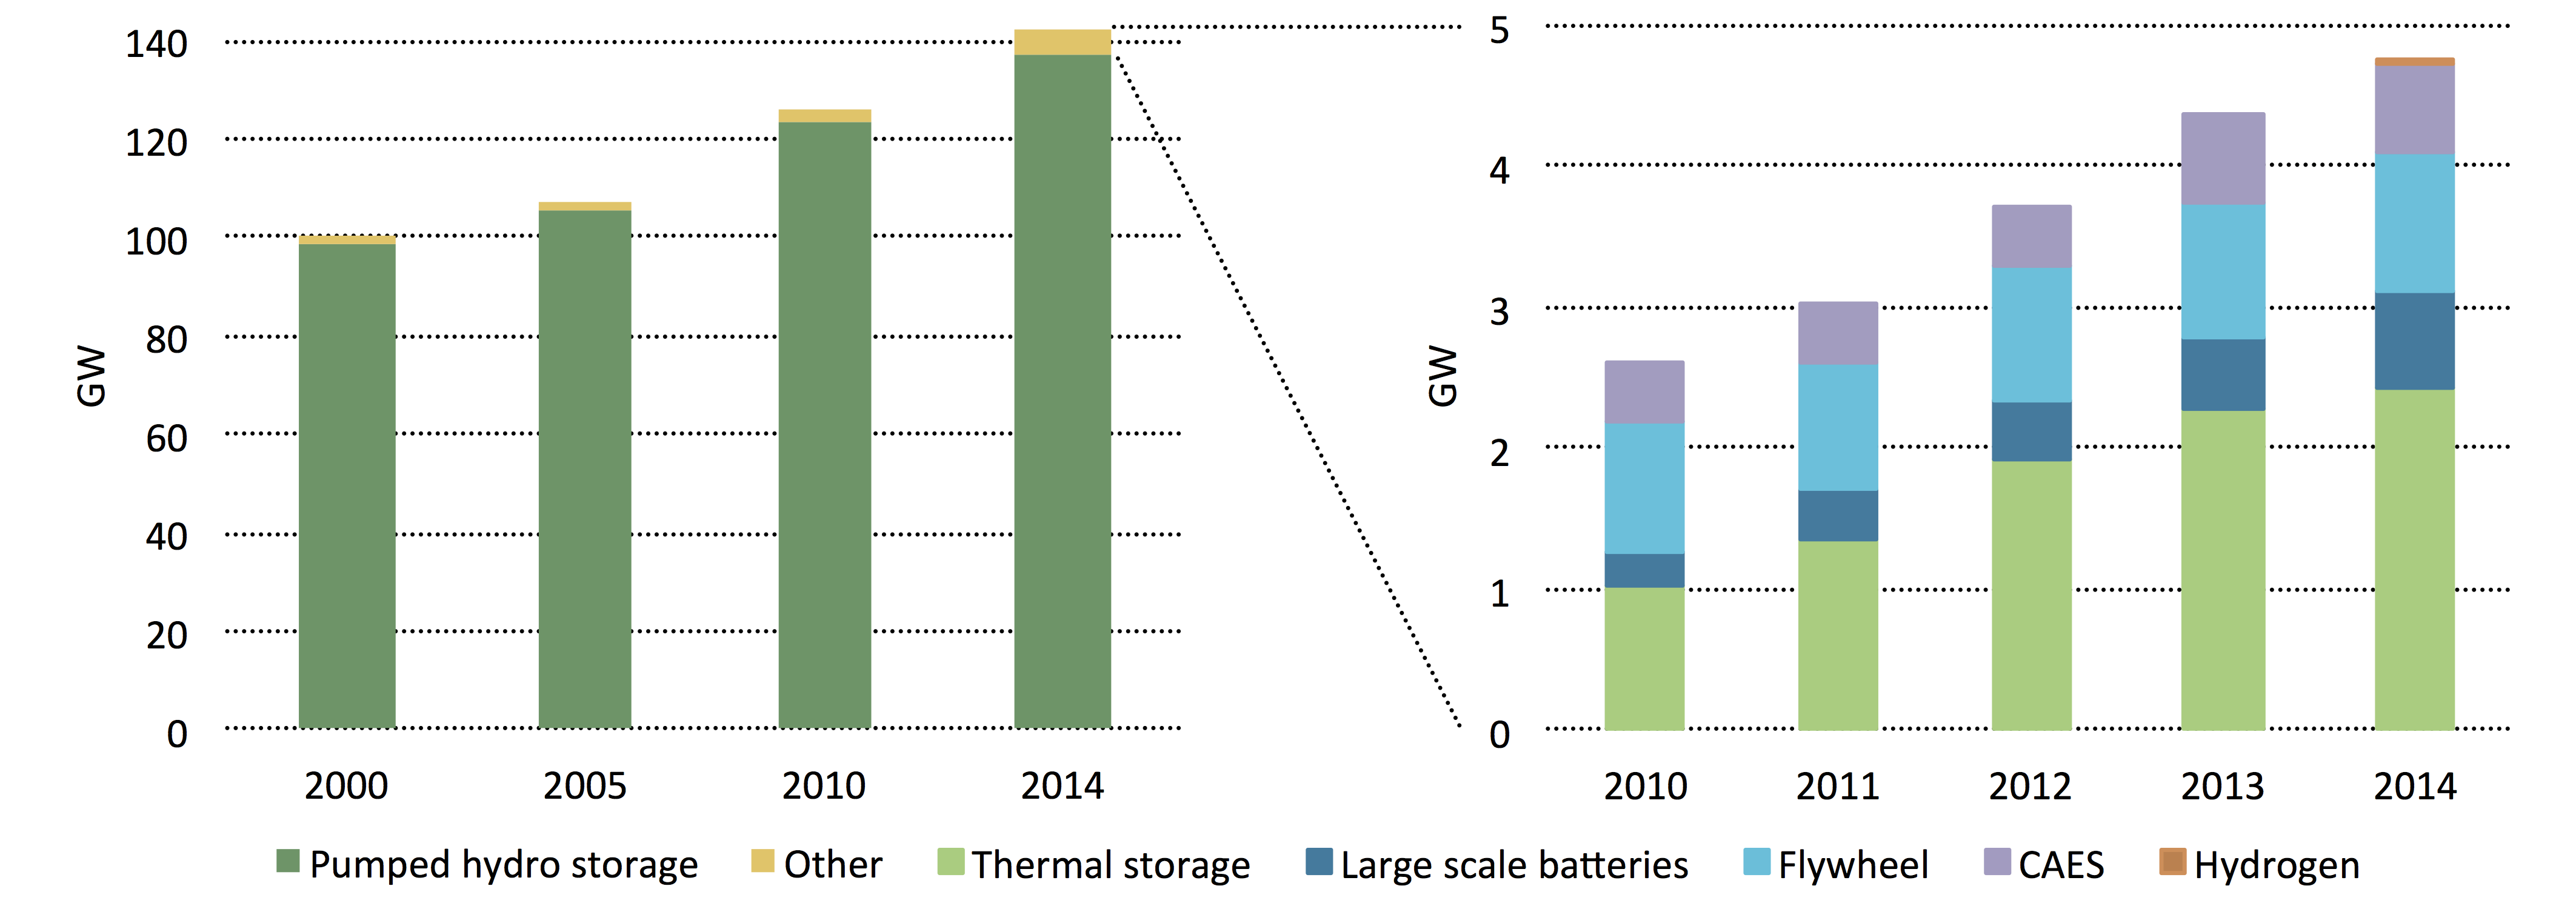
\includegraphics[width=1\linewidth]{FIG/EESgridCapacity}
\caption[Worldwide installed capacity for grid connected storage.]{Worldwide installed capacity for grid connected storage \cite{IEA2015}.}\label{EESgridCapacity}
\end{figure}
For supporting the PV system by supplying the prescribed load curve, the EES requires a Power output of about \SI{100}{\mega\watt} and a storage capacity from several hours. Therefor not many technologies comes into question. Figure~\ref{EEStechnologies} shows that just four EES technology fields could meet the requirements of the prescribed load, namely pumped hydroelectric storage (PHS), compressed air energy storage (CAES), hydrogen (H\textsubscript{2}) storage and battery storage.

The PHS technology is fully mature and reaches efficiency ranges of \SIrange{70}{85}{\percent} with lifetimes between 20~000 and 50~000 cycles \cite{IEA2014c}. But the applicability of this technology is required by potential energy of the storage medium and is therefore highly limited by the regional landscape and there differences in altitude. Furthermore is the apply of PHS in desert regions not well located due to high evaporation losses.

The overall storage efficiency of the H\textsubscript{2} storage is below \SI{40}{\percent} and mainly still in demonstration stage \cite{IEA2014c,IEA2015}. Therefore this technology is also not suited for a adaption to a PV system.

\begin{figure}[htbp]  
\centering
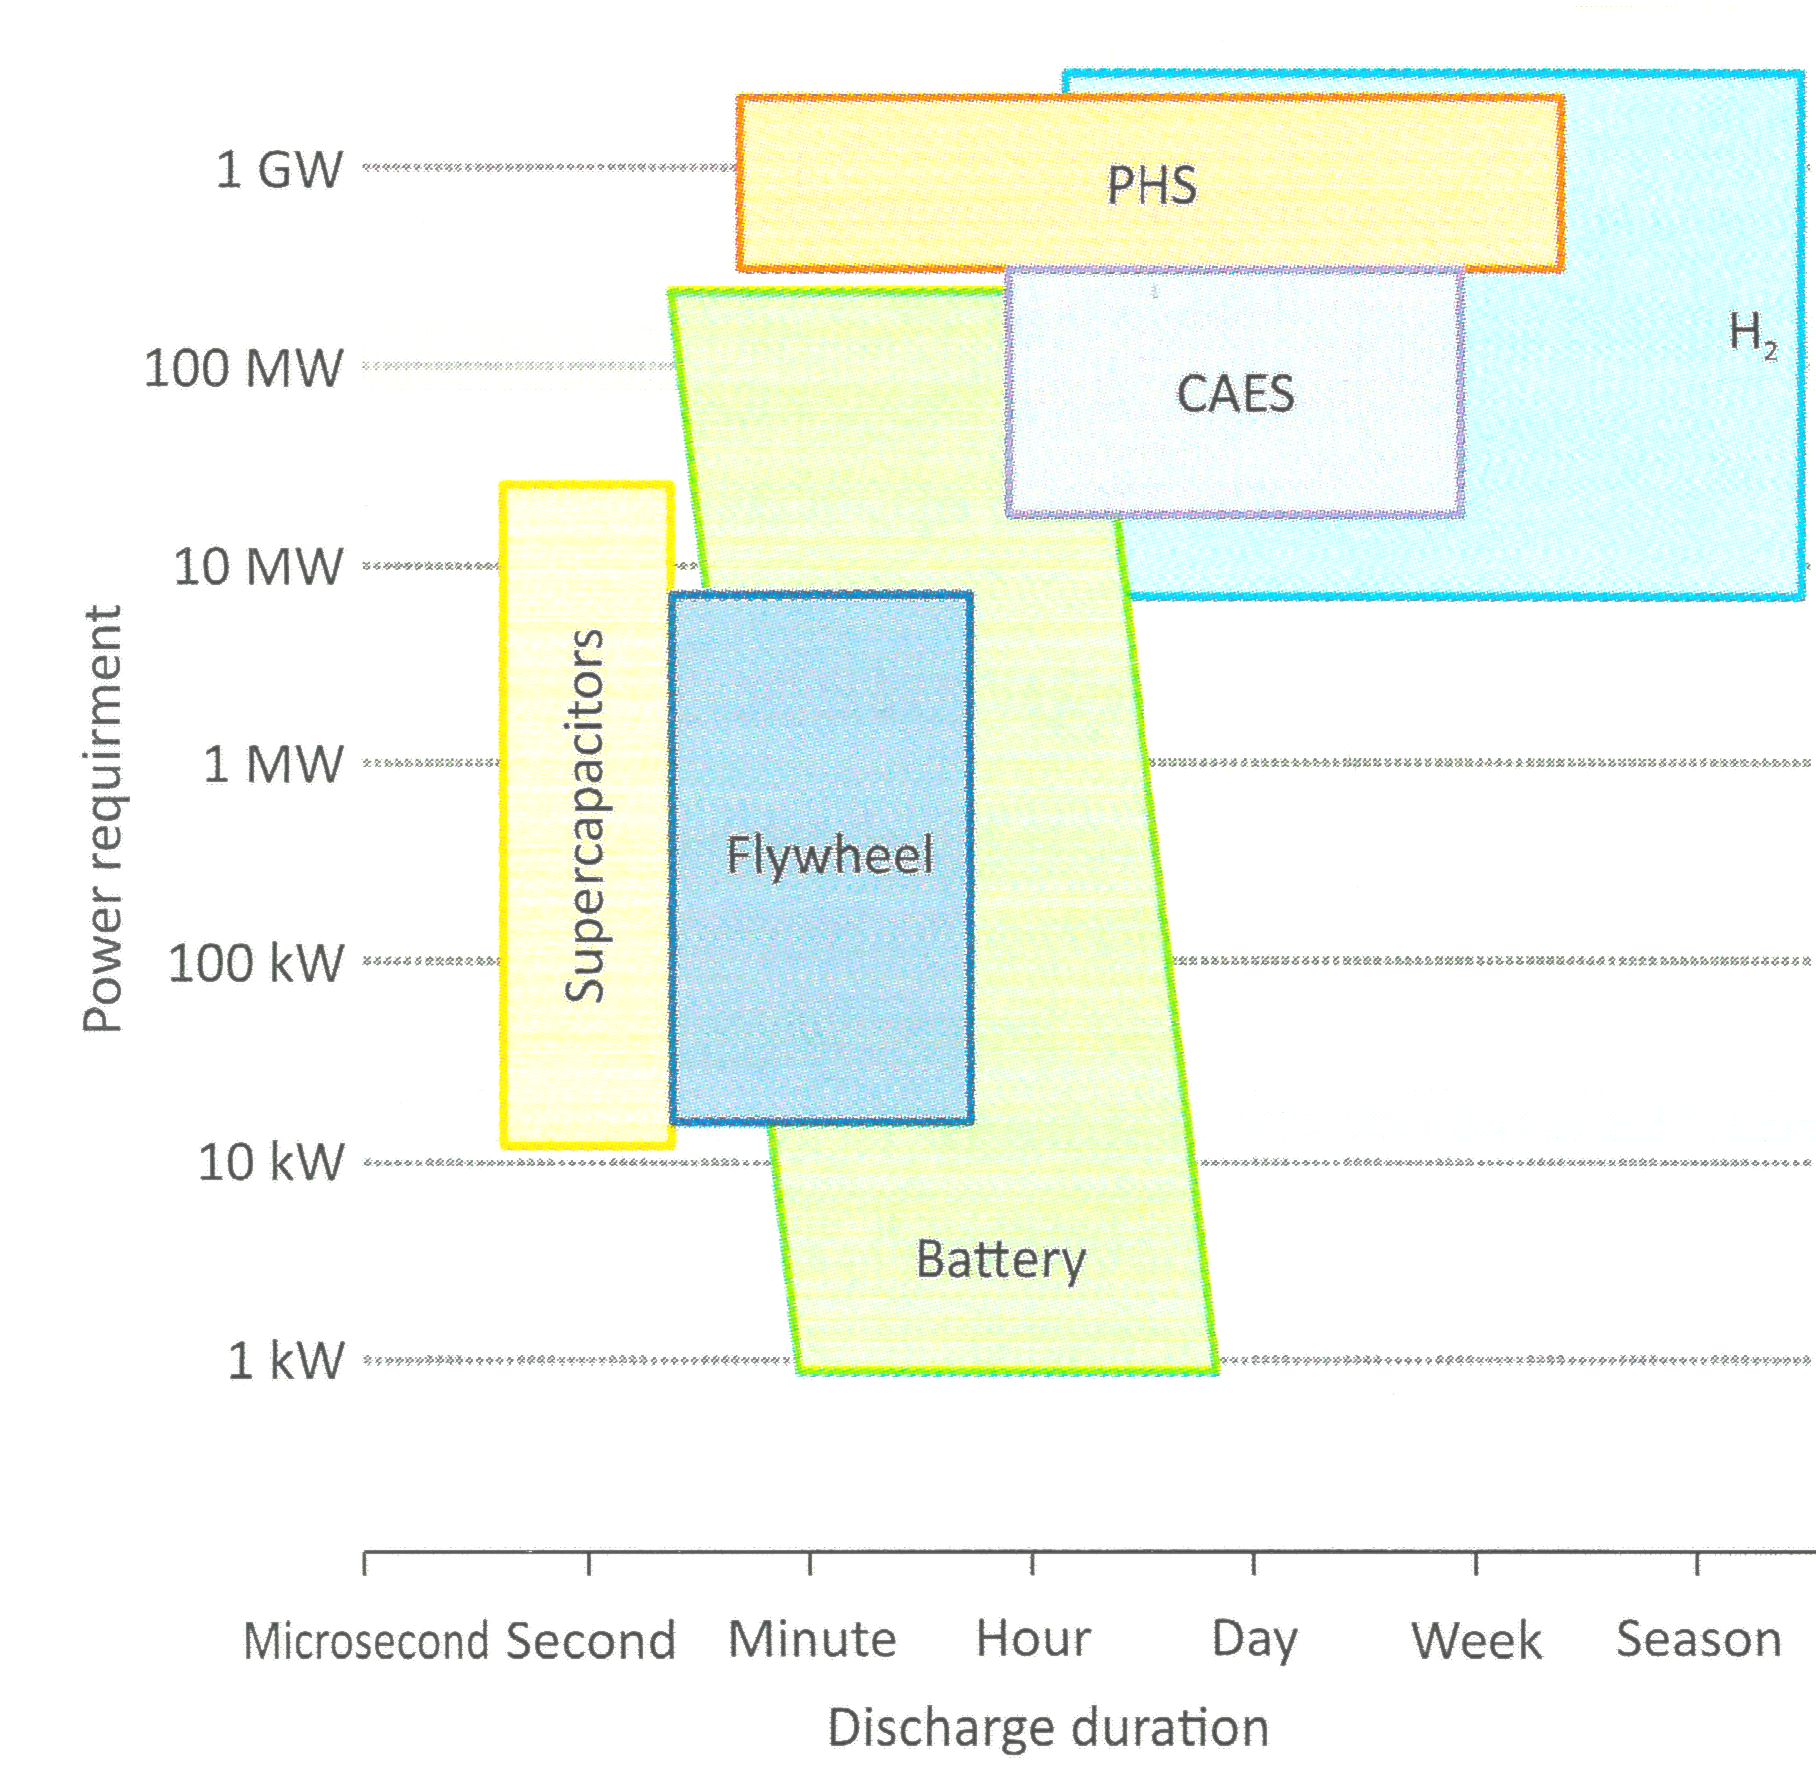
\includegraphics[width=0.6\linewidth]{FIG/EEStechnologies}
\caption[Energy storage technologies ranges.]{Energy storage technologies ranges \cite{IEA2014c}.}\label{EEStechnologies}
\end{figure}
The CAES technology is at a deployed maturity stage and has a for the application as PV system adapted EES a suitable capacity range of \SIrange{100}{300}{\mega\watt}. Also the cycle lifetime of 10~000 to 25~000 cycles is convincing. But with a range of \SIrange{50}{75}{\percent} efficiency, it would have had to high losses, which must be compensated by a oversized PV system. Thererfor is CAES not applyed in the subsequently comparision.  \cite{IEA2014c}

Battery storage technology includes different battery technology types, which also distinguish there own individual specifications by fabrication disparities. Most worth mentioning are Lithium-ion (Li-ion) battery with a overall efficiency of \SIrange{85}{95}{\percent} and a lifetime of 1~500 to 10~000 cycles, sodium–sulfur (NaS) battery which has a efficiency range of \SIrange{75}{90}{\percent} at 2~000 to 5~000 cycles, vanadium redox flow battery (VRB or also called VRFB) at a overall efficiency of \SIrange{65}{85}{\percent} and a lifetime of more than 10~000 cycles and lead–acid (LA) battery usally has a overall efficiency of \SIrange{65}{85}{\percent} at a lifetime of 2~000 to 10~000 cycles. \cite{IEA2014c,Zakeri2015}

It can be seen that a battery storage is a suitable solution for adaption to a PV system. But it must be noted, that the cycle lifetime of all batteries is highly effected by the charging and discharging settings and can thereby vary a lot.

The spread of total capital costs of the different EES technologies can be seen in Figure~\ref{TCC_EES}. It is striking that the range of costs can be huge and highly depends on the specification of the application.

\begin{figure}[htbp]  
\centering
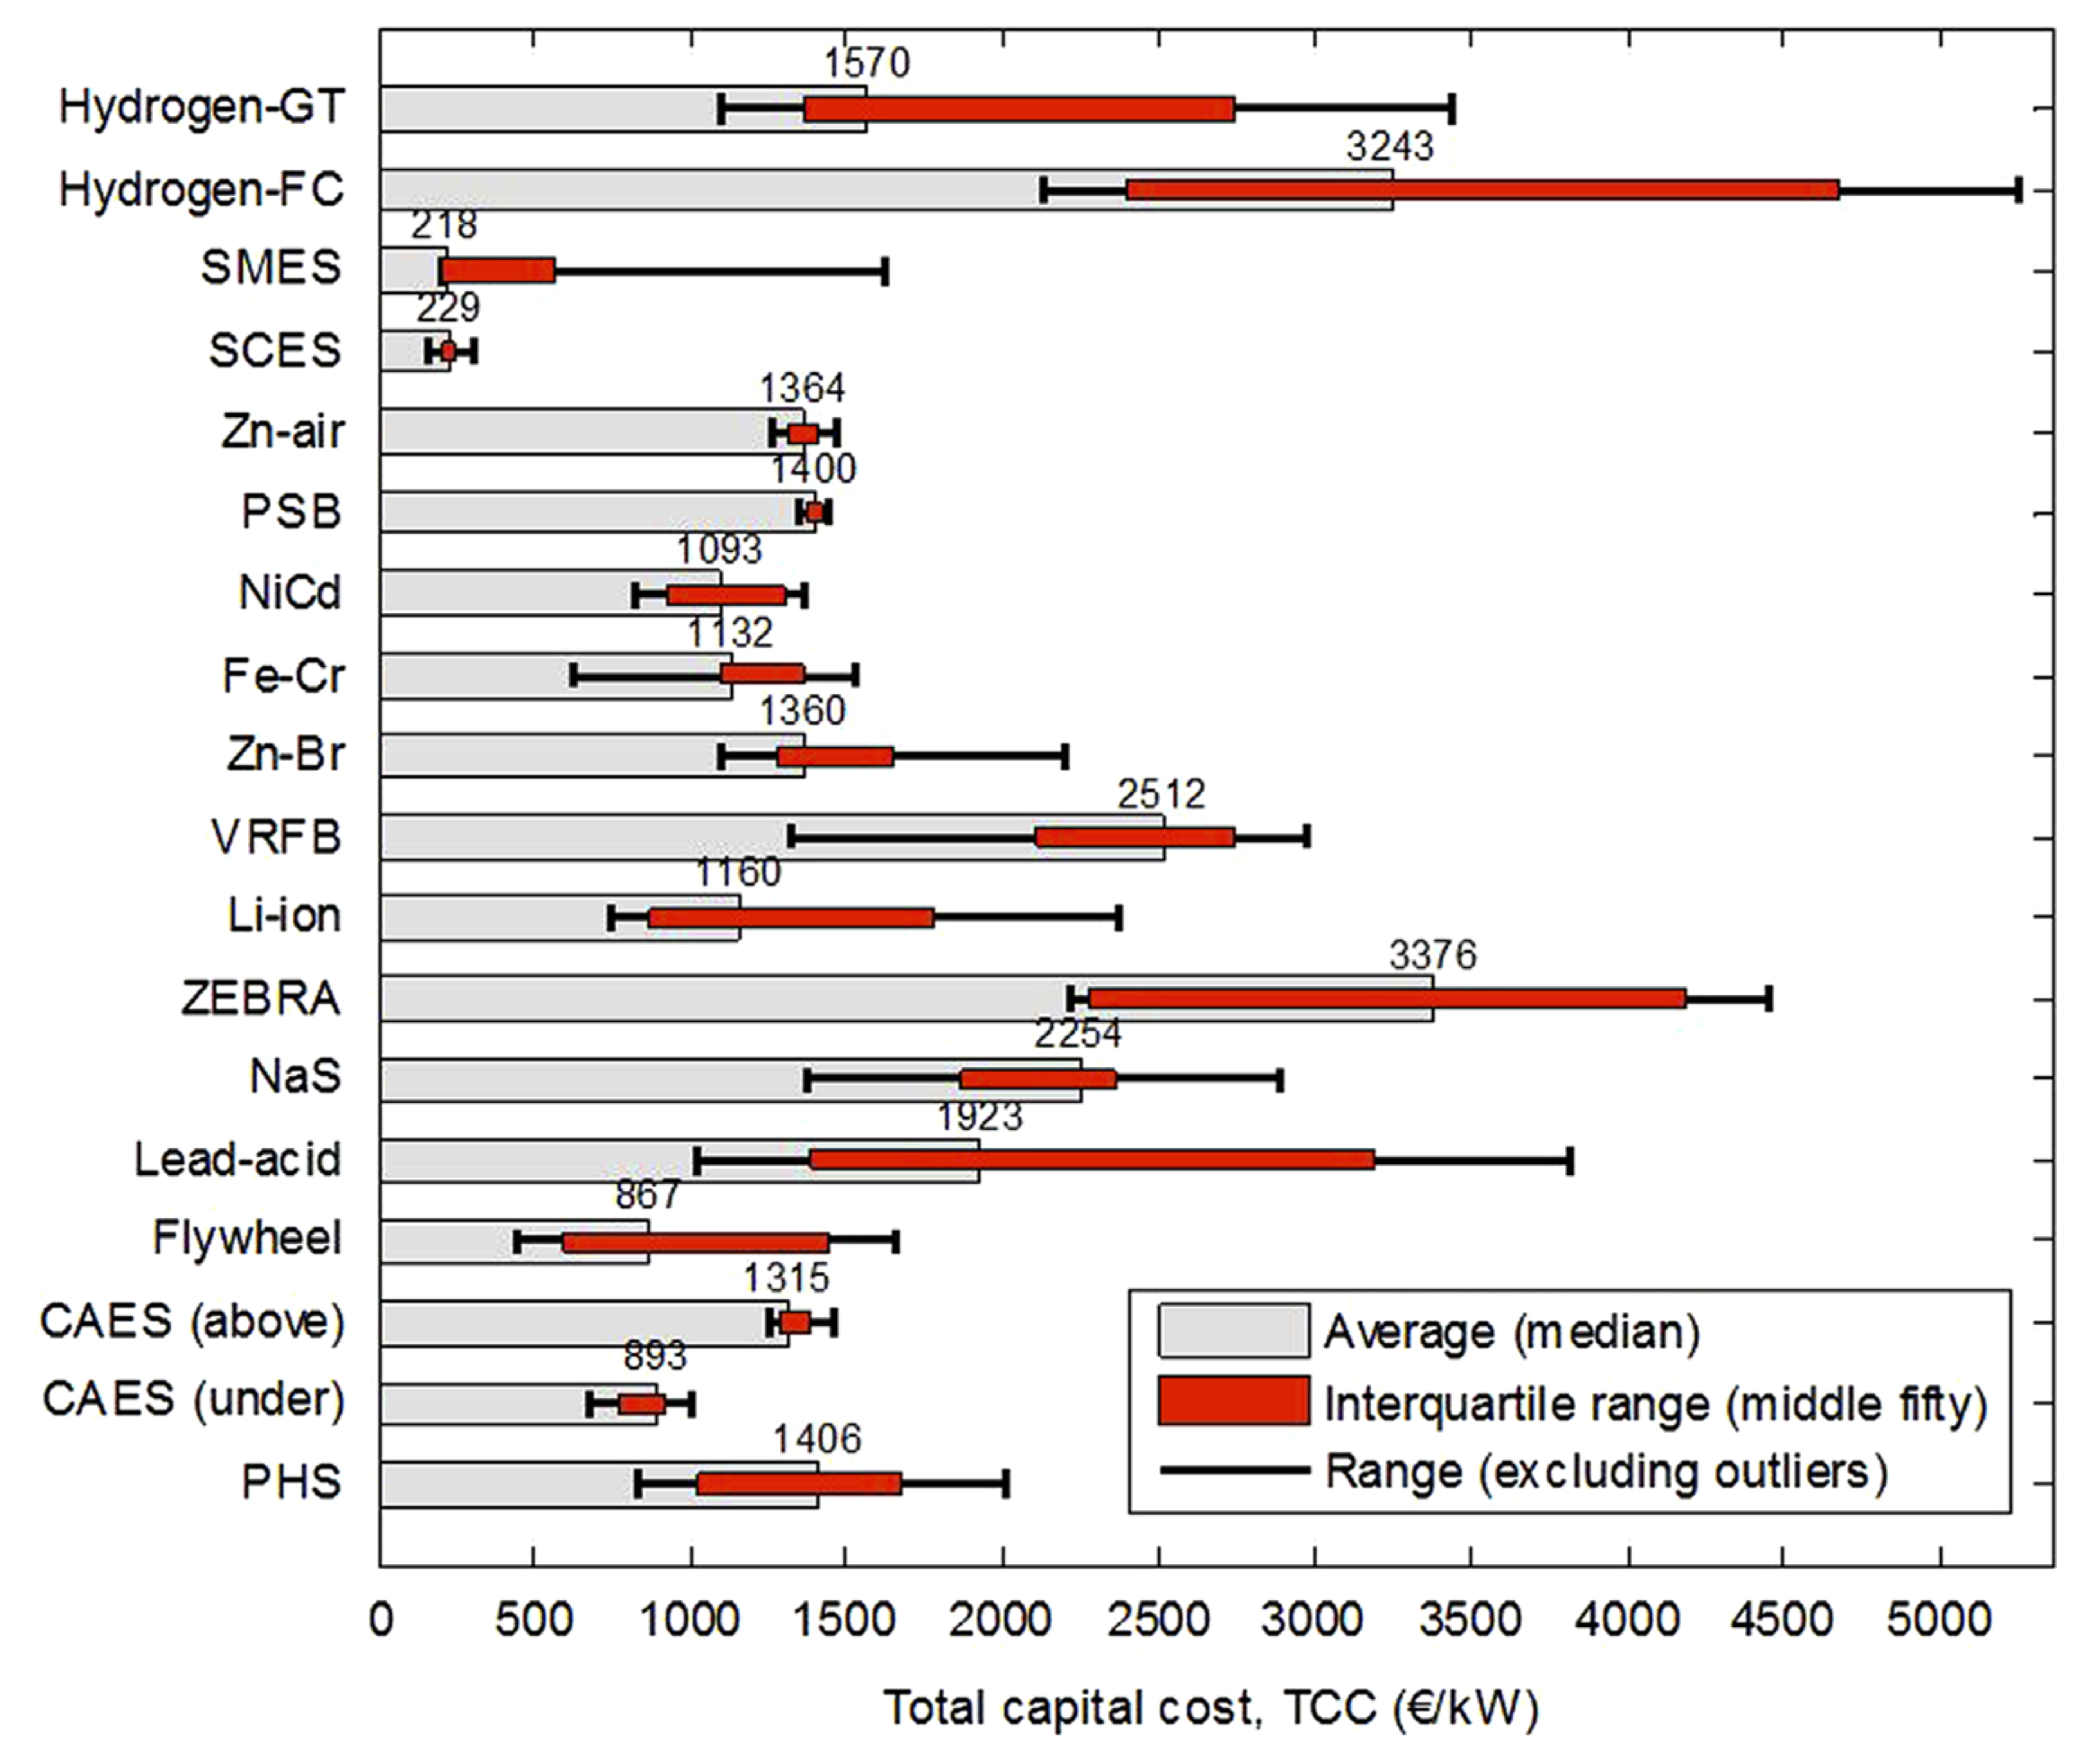
\includegraphics[width=0.65\linewidth]{FIG/TCC_EES}
\caption[Total capital cost in EUR of large-scale EES systems per unit of nominal power rating including costs of power electronics, storage part, fixed obtain and maintainence and maybe incidental replacement costs.]{Total capital cost in EUR of large-scale EES systems per unit of nominal power rating including costs of power electronics, storage part, fixed obtain and maintainence and maybe incidental replacement costs \cite{Zakeri2015}.}\label{TCC_EES}
\end{figure}
\section{Impact of cost of capital on the levelised cost of solar power} \label{section WACC}
Most low-carbon technologies in the power sector, specially solar and wind powered renewable, incur the main part of there cost up-front. They are costly to build but, thanks to cost free renewable source, comparative inexpensive to operate.

The weighted average cost of capital (WACC), which is a mix of the  rate of return on capital and the interest rate for dept, at which the necessary capital and dept can be obtained is a crucial factor shaping the delivered cost of energy from solar technologies. The lower the WACC, the less expansive is energy from solar resources. In turn, factors that increase the WACC drive up the LCOE. In the case of an exemplary PV system, if the WACC exceeds \SI{9}{\percent}, finacing costs begin to dominate the LCOE of PV electricity (see Figure~\ref{WACC}). 

\begin{figure}[htbp]  
\centering
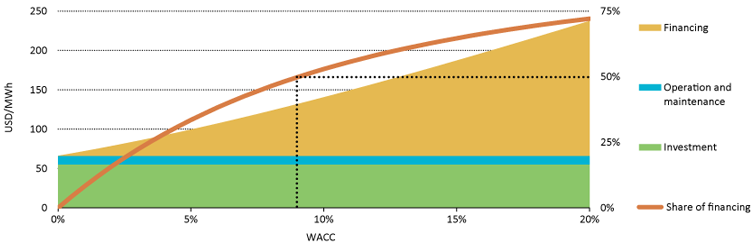
\includegraphics[width=1\linewidth]{FIG/WACC}
\caption[Impact of cost of capital on the levelised cost of an exemplary solar PV systems.]{Impact of cost of capital on the levelised cost of an exemplary solar PV systems \cite{IEA2015}.}\label{WACC}
\end{figure}
Several factors influence the cost of financing. For technically mature technologies, the most relevant risk are those associated with the general investment climate in a market, the maturity of the local supply chain and the off-taker agreements. Depending on the policy, market and regulatory framework, investors may be exposed to substantial risk, which is bound to increase the WACC. \cite{IEA2014c} 

The International Energy Agency calculates there LCOE for solar power applications (CSP and PV systems) with a WACC of \SI{8}{\percent} \cite{IEA2014c}. This also can be assumed for a EES application \cite{Zakeri2015}.

As it was said, the WACC depends from the regional marked. For SA the WACC varied in 2013 from \SIrange{7.93}{8.89}{\percent} for onshore wind applications \cite{IEA2015}. For the subsequently simulation is a WACC of \SI{8}{\percent} for all solar power plants assumed.

\pagebreak
\section{General assumptions for a simulation-based comparison of large-scale solar power plants} \label{General assumptions}
To compare large-scale CSP and PV technologies, a simulated case study was performed on the basis of a CR system, PTC system and a PV system with addapted EES. Specific attention was given to maximizing daytime operation and meeting the prescribed demand curve as it was defined in Section~\ref{SystemloadinSA}. The photovoltaic system was extended with battery storage. The storage capacity allocated for the simulation considerably exceeds the real capacity of electrical storage units currently available and is more than one-sixth the globally installed battery storage capacity of \SI{690}{GW} \cite{IEA2015}. Due to the scale and particularly with respect to the photovoltaic plant, the comparison is theoretical in nature.

With the aim of producing quantifiable and comparable results, the different solar supplied power plants will be simulated under different input  parameters. After that, selected comparable output parameters will be analyzed, evaluated and rated.

The plant technologies selected for comparison are: 
\begin{itemize}
\item CSP molten salt central receiver with thermal energy storage
\item CSP synthetic oil parabolic trough with thermal energy storage
\item PV fixed elevated flat plate collectors with adapted electrical energy storage
\end{itemize}
The PV plant has been extended with a lithium-ion battery storage for the simulation, while the thermal energy storage of the CSP plant uses molten salt technology. All plants were laid out for a maximum net power output of \SI{100}{\mega\wattel}. The plants are driven to match a selected load curve. In order to find an appropriate power plant design to match the load of the scenario, different layout parameters, using various storage and collecting field sizes, were tested. The location and related weather data of Upington was definde and described in Section~\ref{Solar radiation} for this simulation. The solar power plants was implemented and simulated in NREL’s System Advisor Model (SAM) version SAM 2015.6.30 r3 for OS X \cite{NREL2015}. SAM is designed to simulate performance and financial models of different types of renewable energy. For this simulation, only the performance component was used. The financial analysis was done separately. 

The financial parameters and the resulting levelized cost of electricity (LCOE) are calculated separately for all power plants in Microsoft Excel 2011 (vers. 14.5.7) for Mac, using a simplified method which is documented in Appendix~\ref{ChapterLCOE} on page \pageref{ChapterLCOE} using a lifetime of \SI{25}{years} for each plant.